\documentclass[11pt,oneside]{book}
\usepackage{natbib}
\usepackage{color}
\usepackage{amsmath}
\usepackage{amssymb}
\usepackage{graphicx}
\usepackage{epsfig}
\usepackage{amsmath}
\usepackage{amssymb}
\usepackage{shadow}
\usepackage{rotating}
\usepackage{tablefootnote}
\usepackage{tabto}
\usepackage{tikz}
\usepackage{graphicx,wrapfig,lipsum}
\usepackage{caption}
\usepackage{subcaption}
\usepackage{esvect}
\usepackage{hyperref}
\usepackage{booktabs}
\usepackage{Myfullpage}
\usepackage{placeins}
%\usepackage{fullname}
\usepackage{times}
\usepackage{covington}
%\usepackage{mathbbol}
\usepackage{amsthm}
\usepackage{amssymb}
\usepackage{url}
\usepackage{wrapfig}
\usepackage{lscape}
\usepackage{epstopdf}
\usepackage[a4paper, total={6in, 8in}]{geometry}
\geometry{top=2cm,bottom=2cm}
%\usepackage{txfonts}
\usepackage{%
  pstricks,
  pst-node}
\usepackage{fancyhdr}
\usepackage{amssymb,amsmath}
\usepackage{epsfig,graphics}
\usepackage{llncsdoc}
\usepackage{enumerate}
\usepackage{amsmath}
\usepackage{algorithm,algorithmic}

\interfootnotelinepenalty=10000

\renewcommand{\algorithmicrequire}{\textbf{Inputs:}}
\renewcommand{\algorithmicensure}{\textbf{Outputs:}}
% PSTricks settings and definitions
\let\Oldsection\section
\renewcommand{\section}{\FloatBarrier\Oldsection}

\let\Oldsubsection\subsection
\renewcommand{\subsection}{\FloatBarrier\Oldsubsection}

\let\Oldsubsubsection\subsubsection
\renewcommand{\subsubsection}{\FloatBarrier\Oldsubsubsection}

\psset{nodesep=3pt}
% a state of an automaton
\newcommand{\state}[2]{\circlenode{#1}{#2}}
% an initial state: shaded circle
\newcommand{\istate}[2]{\circlenode[fillstyle=solid,fillcolor=lightgray]{#1}{#2}}
% a final state: double circles with a small separating distance
\newcommand{\fstate}[2]{\circlenode[framesep=0pt]{#1}{\pscirclebox[framesep=1pt]{#2}}}
% an initial and final state
\newcommand{\ifstate}[2]{\circlenode[framesep=0pt]{#1}{\pscirclebox[fillstyle=solid,fillcolor=lightgray,framesep=1pt]{#2}}}
% an arc. parameters:
% 1 (optional): 2 angles
% 2: source node; 3: target node; 4: label.
\newcommand{\trans}[4][angleA=0,angleB=180]{\nccurve[#1]{->}{#2}{#3}\Aput{#4}}
\newcommand{\transdash}[4][angleA=0,angleB=180,linestyle=dashed]{\nccurve[#1]{->}{#2}{#3}\Aput{#4}}
\newcommand{\transdot}[4][angleA=0,angleB=180,linestyle=dotted]{\nccurve[#1]{->}{#2}{#3}\Aput{#4}}
\renewcommand{\baselinestretch}{1.67}
\newcommand{\minispace}{\mbox{\hspace{1mm}}}
\newcommand{\smallspace}{\mbox{\hspace{3mm}}}
\newcommand{\bigspace}{\mbox{\hspace{10mm}}}
\newcommand{\textnl}{\textsl}
\newcommand{\naturals}{\mathbb{N}}
\newtheorem{definition}{Definition}[chapter]
\newtheorem{proposition}{Proposition}[chapter]
\newtheorem{lemma}{Lemma}[chapter]
\newtheorem{exa}{Example}[chapter]
\newtheorem{observation}{Observation}[chapter]
\newtheorem{claim}{Claim}[chapter]
\newtheorem{corollary}{Corollary}[chapter]
\newtheorem{theorem}{Theorem}[chapter]
\newcommand{\comment}[1]{}

\newcommand{\edge}[3]{{#1}\buildrel{#2}\over\longrightarrow{#3}}
\newcommand{\transition}{{\bf M}}

\def\ignore#1{}

\begin{document}
\title{\Huge{The ecology of Web browser}
                \huge
             \\[10mm] Sela Ferdman
             \\[25mm] \Large THESIS SUBMITTED IN PARTIAL FULFILLMENT OF THE
             \\       REQUIREMENTS FOR THE MASTER'S DEGREE
             \\[15mm] University of Haifa
             \\       Faculty of Social Sciences
             \\       Department of Computer Sciences
             \\[10mm] November, 2015
}
\author{}
\date{}
\pagenumbering{gobble}
\maketitle{}

\pagestyle{plain}
\pagenumbering{Roman}

\begin{center}
\Huge
     The ecology of Web browser
\huge
\\[10mm] By: Sela Ferdman
\\[3mm] Supervised By: Dr. Einat Minkov and Dr. Ron Bekkerman
\Large
\\ [10mm]THESIS SUBMITTED IN PARTIAL FULFILLMENT OF THE
\\ REQUIREMENTS FOR THE MASTER'S DEGREE
\\ [10mm]University of Haifa
\\ [1mm]Faculty of Social Sciences
\\ [1mm]Department of Computer Sciences
\\ [3mm]November, 2015
\\ [8mm] Approved by:
$\underline{\bigspace\bigspace\bigspace\bigspace\bigspace\bigspace\bigspace\bigspace}$
   \bigspace    Date:$\underline{\bigspace\bigspace}$
\\ (supervisor)\bigspace
\\ [3mm]Approved by:
$\underline{\bigspace\bigspace\bigspace\bigspace\bigspace\bigspace\bigspace\bigspace}$
   \bigspace    Date:$\underline{\bigspace\bigspace}$
\\ (Chairman of  M.Sc Committee) \bigspace

\end{center}

\iffalse
\chapter*{}
\begin{center}
\LARGE{Acknowledgment}
\end{center}
\fi


\newpage
\tableofcontents
\newpage

\addcontentsline{toc}{chapter}{Abstract}
\begin{center}
\title{\huge{
 The ecology of Web browser
\\[5mm]  Sela Ferdman\\
}}
\LARGE{Abstract}
\end{center}

Web browsers are the users window to the World Wide Web. All the web browsers extend their features via addons. There is enormous amount of different addons in the Internet world. A decision whether to install a particular addon is typically in user hands, thus the collection of the user addons is somewhat reflecting the user tastes, domains of interests and other user aspects. And since the collection of addons reflects the user, we can learn the users and try to predict what are the addons that he might have had or what are the addons that are missing in his environment to complete his "personality" profile.
We may call it a user habitat. Given this habitat, we have noticed that the addons have some relations between them and we have hypothesized that by looking at the whole net of users and addons we may find what are the missing elements to complete/stabilize the user habitat. Somewhat like predicting the missing elements in the Mendeleev's table.
Given the data we have about the user,addons and their connections we constructed a big graph with nodes as users, addons and its terms. We have used the Personalized PageRank random walks to traverse the graph and predict the missing addon in the user eco-system. After seeing that our hypothesize is proved correct, we have noticed that there are special relations between addons by some well known companies, like Google, AVG, etc. It turned out that some companies are benefiting from each other - we've indicated this as a symbiotic relations, while other companies are hurt by being in a company with specific company - we've called this a clash relation.
In this work we have developed and proved a methodology to find what addon any given user would be missing. Moreover, we've found a way to uncover hidden relations between companies using the methodology described above.

\listoffigures
\addcontentsline{toc}{chapter}{List of Figures}
\listoftables
\addcontentsline{toc}{chapter}{List of Tables}


\chapter{Introduction}
\pagenumbering{arabic}

Web browsers, a software application for retrieving and presenting resources on the World Wide Web, have become a major component of our everyday environment. As of today, some operating systems are based entirely on browsers (e.g., ChromeOS by Google\footnote{\url{http://www.chromium.org/chromium-os}}). Browser extensions, also called {\it addons}, are computer programs that (as the name suggests) extend, improve and personalize browser capabilities. An extension was developed, for example, that provides visually impaired users with access to the content of bar charts on the Web \citep{elzer2007browser}. Another example addon addresses security concerns, transparently producing a different password for each Website, and by that defending the user against password phishing and other attacks \citep{ross2005stronger}. Toolbars are another kind of a browser extension. These are GUI widgets, which typically reside in the upper part of the browser's window. All major Web browsers support toolbar development as means of extending the browser's GUI and functionality. 

A great number of extensions are installed by users on a daily basis nowadays. It was reported that more than 750 million (non-unique) extensions have been downloaded and installed by users of Google Chrome alone as of June 2012\footnote{\url{http://goo.gl/ggfqxY}}. While browser extensions in general, and toolbars in particular, may be installed following an explicit request by the user, addons are often `silently' installed by a third party as the user downloads some other program from the Web, or likewise are included in a 'software bundle'. There are several reasons why software companies are interested in having specific toolbars installed on the user's machine. First, toolbars are often used for collecting information about the browsing history of the user (e.g., Yahoo! Toolbar). In addition, it is often the case that once installed, toolbar software directs all of the user searches to some dedicated search portal (e.g. MyWebSearch.com). 
The company which owns the Website (and typically also the toolbar) typically receives payments from ad providers (primary ad providers today are Google and Yahoo!), when user clicks on ads presented. Indeed, this model is used extensively nowadays to generate revenue by software companies, which otherwise distribute freeware products \citep{leontiadis2012don}. For example, 45\% of AVG Technologies sales were due to its browser toolbar\footnote{\url{http://goo.gl/ONZ9u}}.  It was estimated that Google, the biggest Web advertising firm, may lose \$1.3 billion in 2013 revenue  due to its toolbar policy changes, which might cause some of the companies to shift to its competitors\footnote{\url{http://finance.yahoo.com/news/google-may-miss-2013-revenue-113926474.html}}\footnote{\url{https://support.google.com/adwordspolicy/answer/50423?hl=en}}.
\iffalse 
Importantly, a user serves as a source of income to the installing party as long as he or she actively uses the toolbar, where users may choose to remove the software from their system anytime. The ability to estimate the period of toolbar ‘survival’ is therefore critical in considering a business model for companies that distribute their software as freeware, counting on revenue generated due to installed toolbars. For example, when a user installs Babylon's translation software , he is offered to install also AVG toolbar, where AVG pays Babylon for these installations. If AVG could estimate whether a specific user would keep its toolbar, it could apply a differential payment model to Babylon according to estimated 'user value'.  In the proposed research, we will consider a large-scale authentic data that tracks browser extensions installed at users' machines on a daily basis. In addition to daily 'reporting', events of adding new browser toolbars are explicitly recorded. Removal of toolbars can be inferred. We are interested in exploring trends in this large-scale data, and in answering specific questions, such as 'can one predict if a particular add-on survives on the user's machine more than K days'. Providing a prediction model of good quality in response to this question is highly valuable to the industry, as discussed above. We will explore machine learning techniques to create prediction models of interest. While many academic studies have used information about user environment towards the creation of user
profiles and personalization of software services, there is no previous research, to the best of our knowledge, which used information about user browser extensions to similarly model user behavior. We will examine the hypothesis by which the existence of an extension on a user’s computer reflects something about the user's
application download history, as well as about his or her general preferences. Specifically, we will evaluate whether clustering users using the underlying data allows one to improve prediction of future behavior. The main research questions and goals are stated in Section 3. An overview of related literature is given below. In addition to previous works on user profiling, we discuss recent learning methods used in large-scale recommendation systems, relating in detail to clustering techniques, which are used to alleviate data sparsity
issues. Finally, descriptions of the prediction models that we plan to use, and an account of the special characteristics and challenges involved with the dataset.
\fi

Often, addons are distributed through the installation process of third-party software products, such as, for example, Adobe Reader. Most of the time, during the software installation process, an opt-out check box is presented to the user per addon to be installed. If the user chooses to uncheck the box, the addon will not get installed. However, many users click through the installation process without reading the small font, and when the process is completed the users discover they installed something they did not intend to. 

Companies that distribute browser addons are engaged in partnerships or compete with each other, such that the Web browser becomes a complex ecosystem similar in its characteristics to the biological environment of the nature. To illustrate this analogy, let us say that addon distributors correspond to biological species. An instance of an addon distributed by company $A$ can be viewed as a subject of species $A$ that coexists in the browser ecosystem with other subjects of the same or different species. Naturally, those subjects can live in symbiosis or in conflict with each other. We observe situations when addons of some companies get installed on a machine together with addons of other companies, which is analogous to a natural migration process when subjects of different species drift together. We also observe clash situations when an addon gets installed on a machine and ``kicks out'' addons of other companies, similarly to a competition phenomenon between different species in the nature. The user (the computer owner) is also playing an important role in the addon ecosystem: some users ``hunt down'' and remove addons that occasionally appear in the computer's browser; other users are more tolerant --- they let addons live in the browser for a long time and do not mind more addons to be installed over time.

[RON: The outline of our findings: In first half of the thesis, we operate on the user level. We use historical data to identify highly probable addons given the collection of addons of a specific user. In the second half of the thesis, we abstract the user data into insights at the addon company level. We identify which addon companies tend to coexist or clash with each other. Both analysis (user-level and company-level) can be used for prediction purposes. Given a specific collection of addons of a specific user, we can make a prediction which addons might get installed on this user's machine. Given two addon companies that were identified as partnering / competing with each other, we can predict their behavior in the future as their addons are evolving.]

[RON: a paragraph about human factor. After all, we are mostly interested in the user who owns the machine and either installs lots of garbage on it or tries to keep it as clean as possible. Who's is more important here - the user who cares about his/her machine hygiene or the bunch of companies that are trying to push stuff on the user's machine? Who's winning?]

[RON: the term ``computer virus'' has existed for a while - the connection between a hardware system (a computer) with a biological system is quite intuitive. However, we go far beyond this - we're investigating biological \_processes\_ in an artificial environment, which sounds pretty novel]


\chapter{Related Research}
\label{sec:related}


\section{User Profiling}
\label{sec:user_profilingg}

User profiles characterize users according to their personal
preferences and skills, as reflected by raw material gathered from
their interaction histories with the system \citep{koch2001software},\citep{gauch2007user}. According to \citep{gauch2007user}, User profiling is typically either knowledge-based or
behavior-based. Knowledge-based approaches engineer static models of
users and dynamically match users to the closest model. In this
paradigm, questionnaires and interviews are often employed to obtain
relevant information about the user. Behavior-based approaches model
user behavior directly, typically using machine-learning techniques,
to discover useful patterns from behavioral data. In particular,
various aspects of user behavior at the desktop are reflected by
browser usage \citep{benevenuto2009characterizing},\citep{bilenko11}. \citep{lieberman1995letizia} and \citep{joachims97} have inferred user preferences given user-browsing behavior. \citep{sugiyama2004adaptive} constructed user profiles based on pure browsing history,
comparing their model with collaborative filtering.  \citep{lu2011learning} developed a set of algorithms to support efficient
learning of user preferences, where the observed data consists of
pairwise comparisons of items.  A general overview of user modeling
techniques can be found in \citep{leontiadis2012don}. \citep{sebastiani02} provides a survey of current machine learning
approaches used for user profiling.  Various learning approaches may
be applied, including Bayesian classifiers clustering, decision trees
and artificial neural networks \citep{pazzani97}, multi-class classification \cite{bauer2014analyzing},
and so forth.  While browsing behavior has been studied in the context
of user profiling, in the proposed research we are interested in using
of a different type of `behavioral logs'. In particular, we believe
that the logs detailing the add-ons installed on the user's machine
over time can be used as another source of meaningful information
about the user's preferences. To the best of our knowledge, this type
of user history data has not been studied before. The user profiling
approach we are interested in is clearly a behavior based
one. Accordingly, we will seek to derive patterns from these data logs
that are meaningful using machine learning methods.

\section{Recommender Systems}
\label{sec:recommender_systems}

Recommendation (or, Recommender) system applications \citep{resnick1997recommender} consider two
classes of entities, usually referred to as users and items. Users
have preferences for certain items, where recommender systems are
aimed at teasing out these preferences out of historical data. The
underlying data corresponds to a utility matrix, assigning values to
user-item pairs that represent what is known about the degree of
preference of that user for that item. In order to construct this
matrix, information need to be first collected on the preferences of
the users for a set of items (e.g., movies, songs, browser
extensions). Such information can be acquired explicitly (typically,
by collecting users’ ratings) or implicitly (typically, by
monitoring users’ behavior, such as songs heard, applications/add-ons
downloaded ,web sites visited and books read).  Recommender systems
produce a list of predictions following one of two main paradigms -
through content-based modeling or collaborative
filtering. Content-based (CB) systems examine properties of the items
and determine inter-item similarity based on their properties. Past
predictions are then projected onto similar items. For example, if a
Netflix user has watched many sci-fi films, then the system would
recommend other movies of the sci-fi genre in the database. In a
content-based system, one must therefore construct for each item a
profile, which is a record representing important characteristics of
that item. Items profiles can be described by vector of Boolean, as
well as multinomial or continuous values. It is possible that item
features be obtained automatically from tags \citep{golder2006usage}. One of the earliest
attempts to tag massive amounts of data was the site del.icio.us,
later bought by Yahoo!, which invited users to tag Web pages. Notably,
browser extensions are often assigned tags by its developers, tags
like Sports, Weather Forecasts, Games and Entertainment.
Collaborative-Filtering (CF) systems (term coined by \citep{goldberg1992using}) focus on the relationship between users and items. They
use the known preferences of a group of users to make recommendations
or predictions for other users, based on their similarity to the
identified user groups. That is, past actions of a group of users are
tracked in order to make predictions for individual members of the
group. The biggest advantage of collaborative-filtering systems over
content-based systems is that explicit content description is not
required. Two main types of algorithms for collaborative filtering
have been researched: memory-based and model-based.  Memory-based CF
approaches assess inter-user similarity based on common items in the
user-item matrix. These approaches are often deployed into commercial
systems (e.g. Amazon ) because they are easy-to-implement and highly
effective \citep{vapnik1999overview}. However, there are several limitations of the
memory-based CF techniques, such as the fact that similarity
assessments are unreliable when data is sparse and the common items
are few. In order to overcome these shortcomings, model-based CF
approaches have been developed. Model-based techniques use the
collected data to estimate, or learn, a model to make predictions
\citep{breese98}. Well-known model-based CF techniques include Bayesian belief
nets (BNs) \citep{breese98}, as well as use of clustering \citep{ungar1998clustering},\citep{zhu2009analyzing} and latent
semantic analysis \citep{hofmann2004latent}. While memory-based techniques alleviate data
sparsity issues, they involve an additional expense of model-building.
Hybrid techniques, such as the content-boosted CF algorithm [28] and
the approach by \citep{gong2009combining}, combine collaborative filtering and
content-based techniques, hoping to avoid the limitations of either
approach and thereby improve recommendation performance. \citep{breese98} proposed a probabilistic approach to collaborative filtering,
which computes the probability that user u give a particular rating to
item s given the user’s ratings of the previously rated items. Two
alternative probabilistic models were considered: clustering models
and Bayesian networks. In the first approach, like-minded users are
clustered into classes; given the user’s class membership, the user
ratings are assumed to be independent, i.e., the model structure is
that of a naïve Bayesian model. The second model represents each item
as a node in a Bayesian network, where the states of each node
correspond to the possible rating values. Both the structure of the
network and the conditional probabilities were learned from the
data. Another interesting methodology of adapting the user profile in
a dynamic and automatic way is presented in \citep{marin2013dynamic}.

\section{PageRank}
\label{sec:pagerank_related}
PageRank was originally proposed by Page and Brin~\citep{page1999pagerank} as a ranking system
for Web pages. Over the last decade, PageRank has gained popularity  in a wide range of applications and domains, ever since it first proved to be  effective in determining node importance in large graphs (which was the pioneering idea behind Google's search engine). Page and Brin considered PageRank as a model of user behavior.
\noindent
A simplified definition of PageRank as proposed in \citep{page1999pagerank} is:
\begin{equation}
 PR(u)=\sum_{v\in B_u}\frac{PR(v)}{N_v}
\end{equation}
where $PR(u)$ is the PageRank score of a webpage $u$, $B_u$ is the set of pages that hyperlink $u$, and $N_v$ is the number of hyperlinks from page $v$. This means that pages that link to page $u$ are providing a portion of their PageRank score to the PageRank score of $u$. %A portion of rank comming from a page $v$ pointing to $u$ is equal to all other portions that are provided to other pages which have a link from page $v$. 
This simplified definition of PageRank leads to some problems. It doesn't consider pages with no outgoing links, disconnected clusters of pages with no hyperlinks outside, and loopy hyperlinks over which the PageRank can get infinitely accumulated. That is why an improved model, the \textit{random surfer model}, was introduced. It simulates a surfer who can randomly start at any page and randomly jump to any page if he ends up surfing over a page without outgoing links or a loop. The definition of the model is:
\begin{equation}
 PR(u) = \frac{1-d}{N}+d\sum_{v\in B_u}\frac{PR(v)}{N_v},
\end{equation}
where $N$ is the number of nodes in the hyperlink graph. The parameter $d$ is a damping factor which can be set between 0 and 1 but usually is set to $d=0.85$. In this form the sum of PageRanks from all Web pages form a probability distribution since the sum equals to one. PageRank can also be interpreted as an vector over all pages and form an eigenvalue problem with the normalized adjacency matrix. PageRank of a page can be interpreted as a probability with which a random surfer chooses the page while the damping factor $d$ can be viewed as a probability that the surfer stops following the links on a page and requests a random page instead.

Although PageRank models a random surfer on the web and computes the probability of finding the surfer at any given page, PageRank exists for any graphs and not just the Web graph. When applied to a specific graph, PageRank produces an importance score for each node. Instead of looking at a \textit{random surfer} on the Web, the non-Web PageRank models a random walk on the graph. Random walks are a common technique to analyze graphs, with a rich history predating PageRank \citep{spitzer2013principles}.

PageRank has found a wide range of applications in a variety of domains within computer science such as computer networking, data mining, web algorithms, and distributed computing \citep{cook04,Bianchini05,LangvilleM03}.
PageRank was used in many recommender systems. Given a set of users and a set of items the users can be interested in, a recommender system learns user's personal preferences and suggests items to users based on those preferences. \citep{gori2006random} propose a random-walk based scoring algorithm called Item-Rank, which is then used in a recommender system.

As \citep{franceschet2011pagerank} explains, the purpose of the PageRank ranking technique is to recursively measure the importance of a node in terms of the importance assigned to the nodes linking to it. In \citep{gyongyi2004combating}, the authors propose a TrustRank method based on PageRank to identify web spam. The authors of \citep{morrison2005generank} paper, find PageRank useful for microarray analysis in bioinformatics. The GeneRank method proposed in \citep{morrison2005generank} produces lists of genes that may be relevant to a microarray experiment. GeneRank uses a surfer over known relationships between genes, while the surfer \textit{restarts} with probability proportional to the activation level of the genes in the experiment. Its output is a set of genes \textit{near} the genes with high activation levels. \citep{freschi2007protein} use similar approach to develop ProteinRank, to predict protein functions. \citep{singh2007pairwise} introduces the IsoRank algorithm to identify functionally similar nodes in two different graphs. The usage of PageRank stretches out to non-computer science areas. The authors of \citep{govan2009offense}, for example,  extended the ideas of \citep{keener1993perron} by using PageRank to compute a rank of sports teams.

The exact computation of PageRank vectors requires solving a system of linear equations, which can be computationally intractable for large graphs. There are iterative methods based on matrix multiplication, but for graphs as vast as the Web, this is still unfeasible. Instead, PageRank related methods often use fast approximation algorithms for PageRank, first developed by \citep{andersen2006local} and tightened by \citep{chung2010sharp}.

\section{Personalized PageRank}
Personalized PageRank is an extension of the PageRank algorithm \citep{page1999pagerank}, both of which are based on a random surfer model. In PageRank, the random surfer starts at any node on the graph. At each step, with a probability of $(1-d)$ the surfer moves to one of neighboring nodes, and with probability $d$ teleports to a random node in the graph. This process is repeated until the walk converges to a steady-state. The stationary probability of the surfer reaching a node is taken as the normalized PageRank score of the node. This form of scoring is the most natural case, which does not artificially prefer some nodes over the others.

In contrast, Personalized PageRank (PPR) enables query-sensitive ranking,
in which we can specify a \emph{query node} (or \emph{nodes}, see below) to obtain a ranking that is personalized for the query. PPR is based on the same random surfer model of the original PageRank, except when the surfer teleports, it always prefers the query node $\mathbf{a}_q$. 
Specifically, at each step, with probability $d$ the surfer teleports to $\mathbf{a}_q$ instead of a random node, thus visiting the neighborhood of $\mathbf{a}_q$ more frequently. As a result, the stationary distribution, called a Personalized PageRank Vector (PPV), is biased towards $\mathbf{a}_q$ and its neighborhood, which can be interpreted as a node importance measure specific to $\mathbf{a}_q$.

Generally speaking, a query can comprise a set of nodes $\mathbf{A}_q$ in the
graph, such that---in the event of teleportation---the surfer will jump to any node in $\mathbf{A}_q$. Fortunately, the PPR computation for a multi-node query is no more difficult than the one for a single-node query due to the \textit{Linearity Theorem} \citep{jeh2003scaling}, as the PPV of a multi-node query is a simple linear combination of the individual PPVs of all nodes in the query.

\iffalse 
[RON: this paragraph doesn't belong here]
The main difference between PageRank and Personalized PageRank is that, instead of relying on a uniform damping vector, PPR is relies on a non-uniform damping vector, to put more importance to a given set of nodes~\cite{haveliwala2003topic}. In our particular case, these 
nodes are the addons of a specific user, that is, the 
members of personalized vector $b$. In practice, given PageRank as in equation~(\ref{eq:pr})
			\begin{equation}
				\overrightarrow{v} = \alpha A^{\rm T}\overrightarrow{v}
				+ (1-\alpha)\frac{\overrightarrow{1}}{n}
				\label{eq:pr}
			\end{equation}
the PageRank equation is adapted as follows to compute the Personalized PageRank ~(\ref{eq:ppr_related_work}):
			\begin{equation}
				\overrightarrow{v} = \alpha A^{\rm T}\overrightarrow{v}
				+ (1-\alpha)\frac{\overrightarrow{b}}{||\overrightarrow{b}||_1}
				\label{eq:ppr_related_work}
			\end{equation}
\fi

Personalized PageRank is used in a wide variety of applications, \citep{lee2011random} adopt PPR algorithm for ranking entities according to a given query that is represented as a set of entities in the graph and infer a multidimensional recommendation. Personalized PageRank has been used both for variants of vertex ranking as well as local partitioning by \citep{andersen2006local}, with later refinements \citep{andersen2007detecting} and applications to directed graphs \citep{andersen2007local}. In TwitterRank \citep{weng2010twitterrank}, the authors adapt PPR to identify influential users of the micro-blogging service. They also discover that Personalized PageRank weighting graphs edges by the similarity of user’s topical interests gives better results than just weighting the nodes according to those same interests.In \citep{berkhin2006bookmark}, the authors use Personalized PageRank for computing that thay call a\textit{bookmark-coloring} bookmark-coloring model.This model computes authority weights over the web pages utilizing the web hyperlink structure. ScaleRank, proposed in \citep{hristidis2014efficient}, efficiently compute edge weighted
personalized PageRanka and provides personalized ranking of typed entity-relationship graphs. It was also noted, \citep{sarkar2008fast}, that Personalized PageRank can be adopted to be a good similarity measure on the Web.\\
\iffalse
MOVED HERE: As mentioned before, the algorithms of PageRank and Personalized
PageRank algorithm have been designed so as to improve Web page
rankings. The Personalized Pagerank variant was first suggested in
\citep{brin1998can}, and shortly after, has been explored to
personalize Web search
(\citep{haveliwala2002topic},\citep{haveliwala2003topic},\citep{haveliwala2003analytical}). Nevertheless,
PageRank may be readily applied to arbitrary graphs to produce node
importance scores, and this places PageRank amongst a class of network
analysis techniques \citep{brandes2005network} known as centrality
measures or indices \citep{koschutzki2005centrality}. Similarly,
Personalized PageRank is a general similarity measure in graphs, used
in multiple domains. For example, in \citep{freschi2007protein}, the
authors used the Personalized PageRank model, which they call
ProteinRank, to predict protein functions. ALSO: In Keren's thesis, we have shown that PPR's random walk similarity metric outperforms classical collaborative
filtering and content-based recommendation methods.
\fi
\subsection{Effect of High Degree Nodes on Personalized PageRank}
\label{sec:ppr_high_degree}
The study of large networks is a fairly recent development, and there have been many phenomena shown to be appearing in real-world datasets. One important property is the small-world phenomenon \citep{watts1998collective}, the existence of short paths between any randomly-chosen pair of vertices. Many real-world networks exhibit small-world behavior, and they are characterized by having a low average shortest path length and many dense subgraphs.
Another hallmark of large graphs is the power-law degree distribution. Several groups of authors independently discovered that virtually every large network found in nature exhibits a power-law degree distribution \citep{aiello2001random,albert1999internet}. Our graph also stands in these standards, as shown in \autoref{tab:node_types} and \autoref{fig:power_law_addons}, the addon nodes degree has a power-law distribution and also the small small-world phenomenon holds. In our research, we are experimenting with removing high degree nodes from the graph. In \citep{sarkar2010tractable}, Sarkar proves that removing high degree nodes from an undirected power-law graph involves a very small penalty. The main intuition behind their analysis is that a very high degree node passes on a small fraction of its probability mass to the out-neighbors,
which might not be significant enough to invest computing resources.They argue that stopping a random walk at a high degree node does not change the personalized pagerank value at other nodes which have relatively smaller degree. Similar to our approach, they turn a high degree
node into a sink by removing all the outgoing neighbors and do not change any incoming edges.


\section{Link Prediction in Graphs}
\label{sec:link_prediction}
Link prediction in complex networks has attracted increasing attention from computer science community. Many social, biological, and information systems can be well described by
networks, where nodes represent individuals, and links denote the relations or interactions between nodes. \textit{Link Prediction} attempts to estimate the likelihood of the existence of a link between two nodes, based on observed links and the attributes of nodes \citep{getoor2005link}.
Social network analysis comes up against the missing data problem \citep{kossinets2006effects}, where link prediction algorithms may play a role.In addition, the data in constructing biological and social networks may contain inaccurate information, resulting in spurious links \citep{von2002comparative, butts2003network}. Link prediction algorithms can be applied in identifying these spurious links \citep{guimera2009missing}.Besides helping in analyzing networks with missing data, the link prediction algorithms can be used to predict the links that may appear in networks. For example, in online social networks, very likely but not yet existent links can be recommended as promising friendships. Similar techniques can be applied to evaluate the evolving mechanism for given networks or finding a missing user addon.
A learning algorithm for link prediction, presented in \citep{lao2010relational}, uses random walk processes to define a distribution, rather than some other forms of logical inference, such as belief propagation.It was shown that also personalized PageRank can be used to approximate belief propagation on certain graphs \citep{cohen2010graph}. \textit{Link analysis} exploits the relationship between resources through links and is a well-researched area \citep{henzinger2000link}. In \citep{gyongyi2006link}, link analysis link analysis has been suggested to help fight web spam. The authors of this paper introduced a measurement called \textit{Spam Mass}. It indicates how much PageRank a page accumulates through being linked to by spam pages. The spam mass is computed  by combining two PageRank scores: the regular PageRank score and a biased one. The biased one is computed by assigning a higher weight to a large group of known reputable pages. The absolute mass estimation can then be calculated by taking the difference between the regular PageRank score and the biased one. The relative spam mass estimation becomes the ratio between the absolute estimation and the total PageRank score. This estimation is similar to our estimations that we use in \autoref{chap:Symbiosis}, when looking for sharp changes between companies PageRank scores.

\section{Clustering}

A known issue of Recommender Systems is the `cold-start' problem,
where little historical data is available for new users, or
items. Clustering is often employed to alleviate the cold-start
problem. A cluster is a collection of data objects that are similar to
one another within the same cluster and are dissimilar to the objects
in other clusters \citep{han2006data}. When applied to the domain of Web browsing
history, clustering can group together a set of Web pages with similar
contents, and users with similar navigation behavior or navigation
sessions. Ungar and Foster \citep{ungar1998clustering} clustered users and items separately
using variations of k-means and Gibbs sampling \citep{geman1984stochastic}, grouping users
based on the items they rated and items based on the users that rated
them. Using to their model, users were re-clustered based on the
number of items they rated, and items were similarly
re-clustered. Each user was assigned to a class with a degree of
membership proportional to the similarity between the user and the
mean of the class. Their recommendation performance on synthetic data
was good, but not as good on real data. A flexible mixture model (FMM)
extends existing clustering algorithms for CF by clustering both users
and items at the same time, allowing each user and item to be in
multiple clusters and modeling the clusters of users and items
separately \citep{si03}. Experimental results show that the FMM algorithm has
better accuracy than the Pearson correlation-based CF algorithm and
aspect model \citep{hofmann2004latent}. Clustering for both users and items is often
referred to as multi-way clustering \citep{bekkerman05} or bi-clustering \citep{zhu2009analyzing}.
Bekkerman at \citep{bekkerman05} have shown that clustering users and items
simultaneously provides better results (when the users and the
features are inter-dependent). In our focus domain, for example, a
user may use one set of browser add-ons for work and another for
entrainment. Multi-Way Distributional Clustering (MDC) is an efficient
implementation of Combinatorial Markov Random Fields (Comraf), a novel
type of undirected graphical models due to \citep{bekkerman2006semi}]. The
model is grounded on three principles: (i) Exploiting multi-modality
of the data, i.e. the fact that the data can be viewed from different
angles or perspectives. For example, consider a dataset of documents
that should be clustered into topics. Rather than represent full
documents, a different modality of this data would be sets of words
that are contained in the documents. Additional modalities would be a
set of author names, a set of documents titles etc. Comraf allows one
to simultaneously cluster a number of data modalities, having each one
potentially improves the quality of all the others. (ii) Most existing
clustering methods are based on explicit definition of a pairwise
distance measure between data instances. Such a measure is usually
chosen heuristically, and can in some cases be inappropriate for
particular tasks. MDC refrains from such an explicit definition and
instead optimizes a global objective function over the entire
data. (iii) Most existing clustering algorithms are either
agglomerative (start with small clusters and merge them to compose
larger clusters), divisive (start with one large cluster and split it
to obtain smaller clusters), or flat, such as k-means (start with k
clusters and rearrange data within these clusters). \citep{bekkerman05} propose to combine all the three approaches together, while
choosing the most appropriate one for each data modality. A detailed
description of the Comraf model is given in \citep{bekkerman2006semi}, and
the underlying clustering algorithm (MDC) is described in \citep{bekkerman05}. Some modalities may be not clustered by Comraf, as explained
in \citep{bekkerman2007multi}.  In the proposed research, the underlying
data is highly sparse. We will therefore explore clustering of items
(add-ons) in order to get denser historical records for each user. In
addition, we may cluster users, in order to associate new users who
have little known history with relevant user groups. As described
above, concurrently clustering data along both dimensions may be
desired.

\chapter{Problem definition}

This is essentially equivalent to the research goals.\\
We have decided to investigate the browser ecosystem from three points of view:\\
1. We simulated an artificial extraction of an addon from its habitat, and we see that the rest of the system works to bring it back.\\
2. We see that some addon "species" (i.e. companies) compose a symbiosis, while others clash with each other (which results in extinction of one of the species).\\
3. We observe how the browser ecosystem evolves over time.\\
Given a successful resolution of first problem, the system can infer what addon is "missing" in current user addons ecosystem and thus predict/recommend an additional addon.\\
As for the second problem we were investigating, these days it becomes more and more relevant. See, for example, recent discovery about SuperFish security breach is a good example about two companies having a major symbiosis (SuperFish and Komodia) and SuperFish and all major anti-viruses addons is a good example of a clash between two companies.\\
It is also interesting to see how the addons in browser ecosystem evolve day by day.



\chapter{Data}
\label{sec:datasets}

%\section{Data}
\iffalse
\textcolor{green}{\textit{Einat:
Describe here the data that we've used. How it was extracted, relevant
statistics (how many users, time span, distribution of addon nunber
per user).. the types of information that we have about each addon
(add-on name, description.. -- include examples). Discuss the issue of
versioning -- there are often small lexical differences between
add-ons, in particular, in version number, but essentially it is the
same addon.}}
\fi

We experiment in this study with large-scale authentic data.  The data includes the list of addons installed on real users' computers over time, collected from users that have agreed to anonymously share this information.  The list of browser add-ons installed on every user's machine is reported in a daily resolution.  This large-scale data is stored using a relational database in cloud at Amazon RDS, and included over 1.5 billion records in 2014. The database is comprehensive, in the sense that it  reports the addons installed in multiple browsers, including Microsoft Internet  Explorer, Mozilla Firefox and Google Chrome. It  is a common scenario that user has more than one browser. ( Since Internet Explorer usually comes pre-installed, many users install an additional browser (typically Chrome or Firefox.) In addition, the users are from all around the globe. 

Our focus is on {\it user}, and {\it addon} tables. Following is a description of the main attributes known for these objects,

{\it Users.} A user record specifies his origin: IP, ISP and Country, as well as the Operating System installed on his computer (i.e. Windows XP, Vista, etc.).

{\it Addon.} The installed add-ons are listed per user. Figures \ref{fig:db_addons_snapshot} and \ref{fig:db_addons_snapshot_desc} include the records per an individual user on a specific date, in which he had Conduit, Skype and Babylon addons installed. As shown in the figure, the following attributes are specified for each add-on:
\begin{itemize}
\item Add-on type: extension, bho, toolbar, etc. (see Type column in the table)
\item The name of the program. (Name column)
\item The full path where it resides on the user's machine. (FileName column)
\item A textual description of the add-on. (Description column)
\end{itemize}

\begin{figure}[t]
\centering
\begin{small}
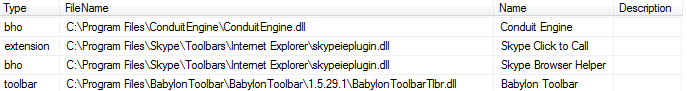
\includegraphics[scale=.8,angle=0]{figures/db_addons_snapshot.png}
\end{small}
\caption{User addons record}
\label{fig:db_addons_snapshot}
\end{figure}

\begin{figure}[t]
\centering
\begin{small}
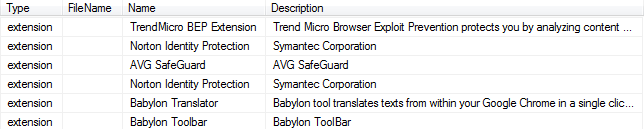
\includegraphics[scale=.8,angle=0]{figures/db_addons_snapshot_desc.png}
\end{small}
\caption{User addons record}
\label{fig:db_addons_snapshot_desc}
\end{figure}

The field values correspond to raw information extracted from the users' machines. Accordingly, it lacks normalization. Figures \ref{fig:addons_versioning_snapshot} and \ref{fig:addons_versioning_snapshot_desc} illustrate the variability across records, which we consider to be co-referent as they describe the same addon. As shown, there are differences across individual records with respect to the path in which the add-on is installed on the local machine, as well as the version number (e.g., 1.8.7.2 vs. 1.8.4.9 in the \autoref{fig:addons_versioning_snapshot}), name and description. Furthermore, the user base is international, and is accordingly multi-lingual.   Typically an addon in Internet Explorer has atleast a path attribute, while addons in Mozilla Firefox and Google Chrome browsers have at least a name attribute. In most cases one of the addon attributes is reported empty.

\begin{figure}[t]
\centering
\begin{small}
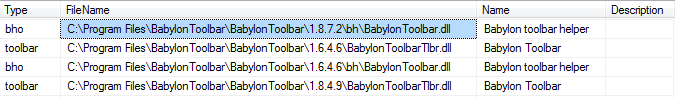
\includegraphics[scale=.8,angle=0]{figures/addons_versioning_snapshot.png}
\end{small}
\caption{Addon with different versions in user record}
\label{fig:addons_versioning_snapshot}
\end{figure}

\begin{figure}[t]
\centering
\begin{small}
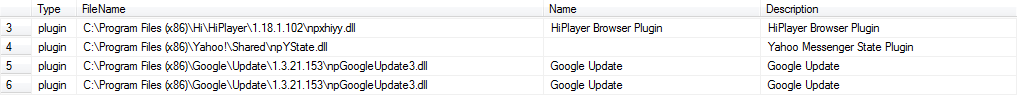
\includegraphics[scale=.8,angle=0]{figures/addons_versioning_snapshot_desc.png}
\end{small}
\caption{Addon with different versions in user record}
\label{fig:addons_versioning_snapshot_desc}
\end{figure}

Finally, we note another characteristic of interest of this data.  Since the add-ons lists per user are updated on a daily basis, it is straightforward to derive add-on changes (installation and removal) over time. However, there is no tracking of user actions or other programs actions. It is therefore impossible to determine which party initiated any of the status changes; for example, we cannot infer whether a particular addon has been removed (or installed) by the user or automatically, by hostile/protecting program. 

\section{Experimental data}

For the purposes of this study, we consider a subset of the data, including all of the records collected over a  period of two months between Aug. 1 2013--Oct, 1, 2013. Overall, this dataset contains 17,942,715 daily user--add-on associations. It consists of 907,844 unique users and 456,458 unique addons. Figure \ref{fig:user_addons_histogram} shows the distribution of the number of add-ons installed daily per user. As shown,  most users have between 9 and 21 addons installed on their PCs.

\iffalse
\begin{figure}[t]
\centering
\begin{small}
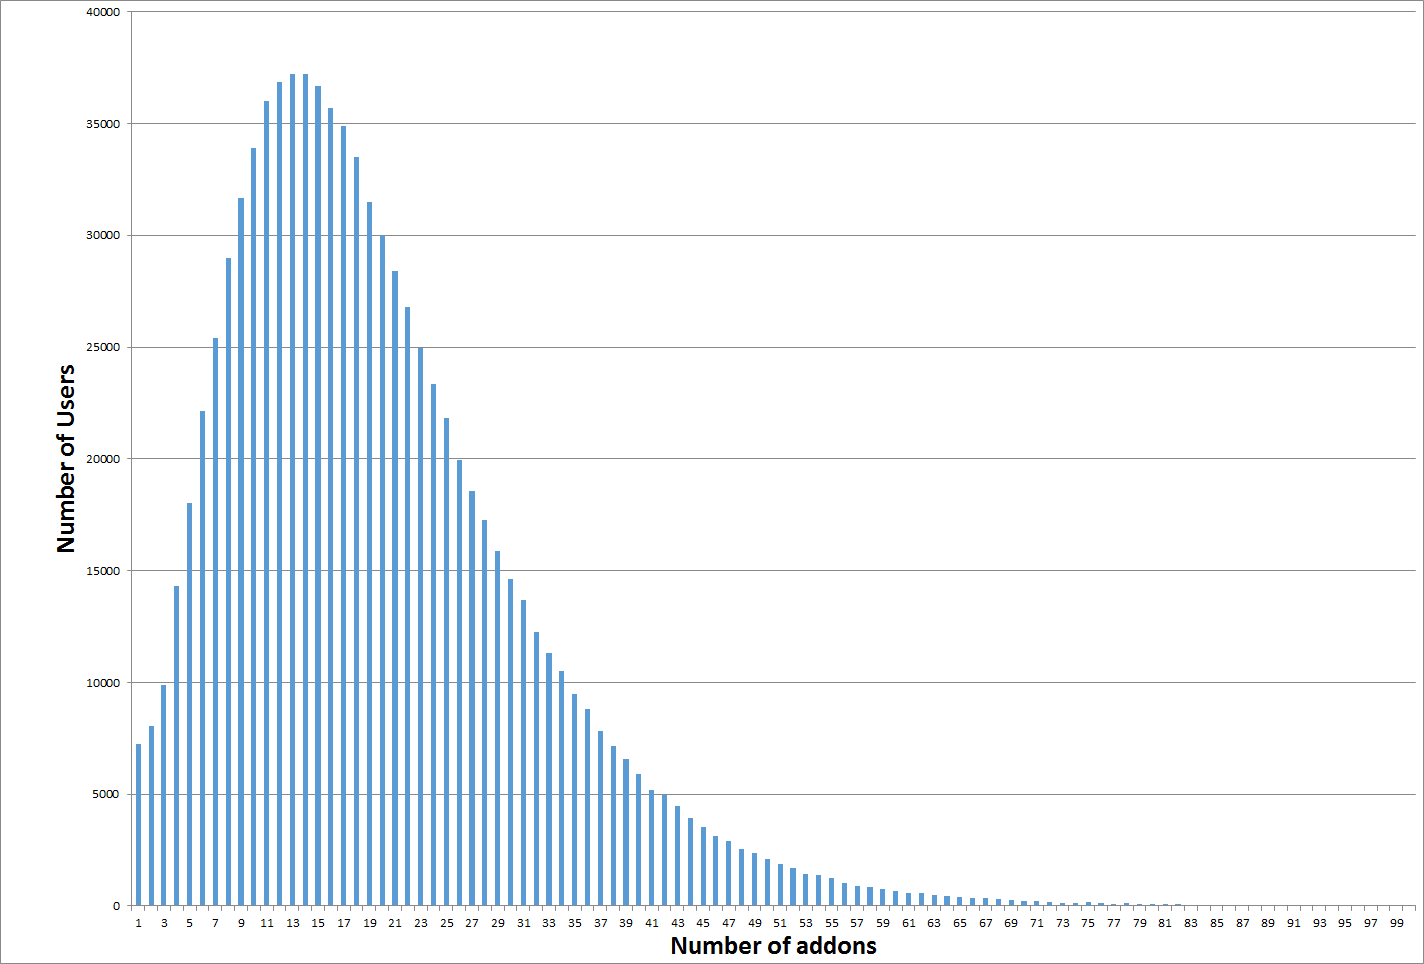
\includegraphics[scale=.9,angle=0]{figures/user_addons_histogram.png}
\end{small}
\caption{Distribution of number of addons per user}
\label{fig:user_addons_histogram}
\end{figure}
\fi

\begin{figure}[!htbp]
\centering
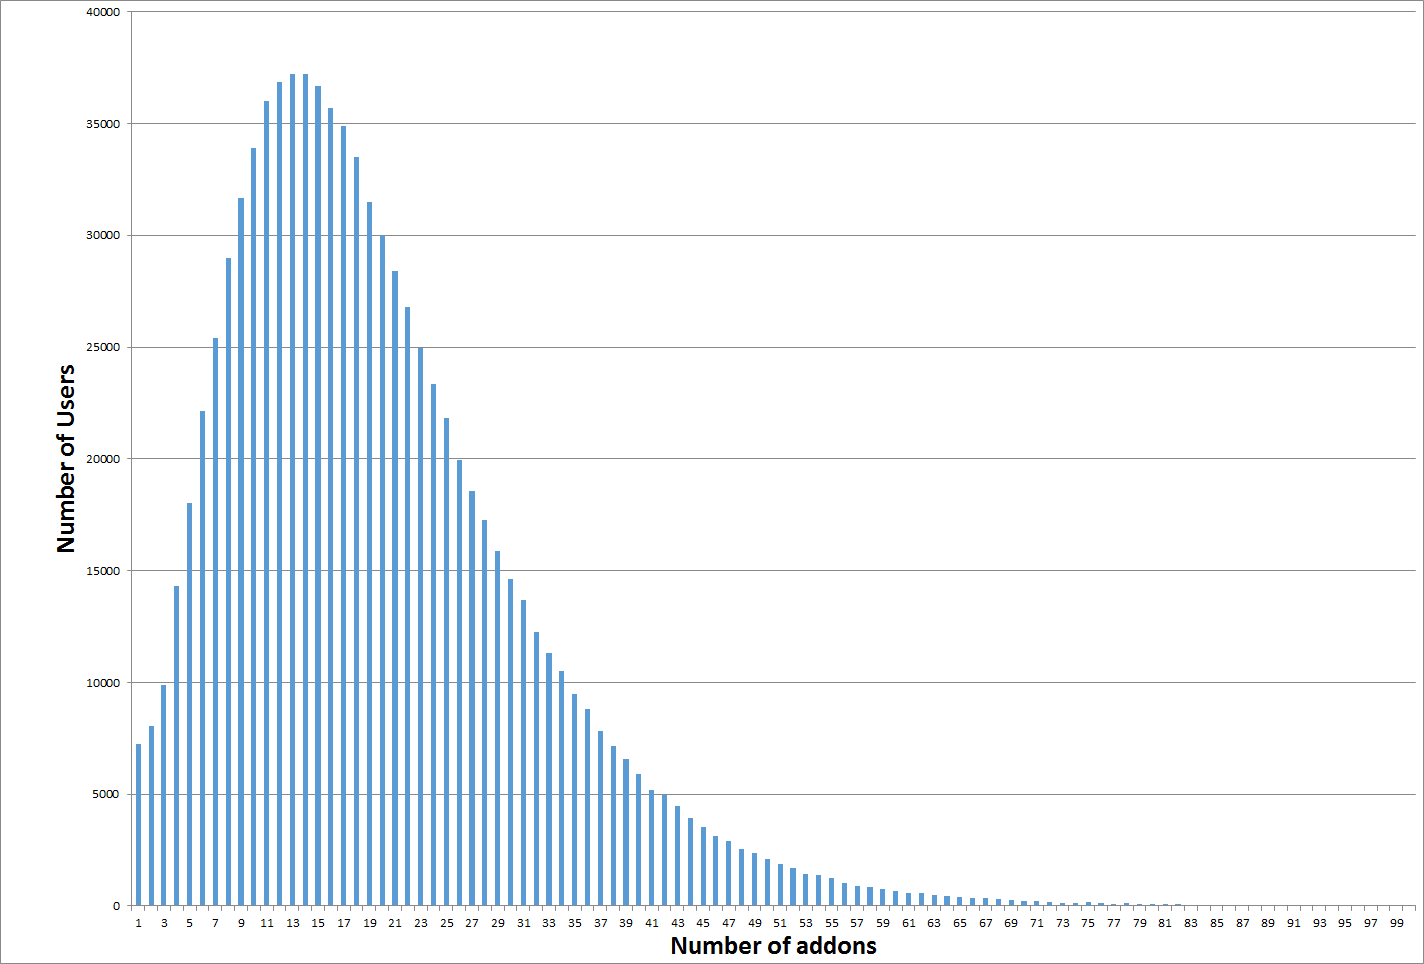
\includegraphics[width=\linewidth]{figures/user_addons_histogram.png}
\caption{Distribution of number of addons per user}
\label{fig:user_addons_histogram}
\end{figure}

In order to enable assessment of textual similarity for record co-reference purposes, we further processed the fields describing each add-on mention into a Bag-Of-Words. These words are represented using {\it terms}, a lexical object type. Given a text string, it is first tokenized, and text cleanup and normalization steps are then applied. For example, we remove non-ASCII characters that serve for encryption purposes on the server. Likewise,  Windows shortcuts for full paths are removed (e.g., VIDEOD$\sim$1 and VIDEOD$\sim$2 and VIDEOD denote the same path), and so forth. Finally, all strings are transformed to lower case, since capitalization is meaningless in this context. Overall, 167,512 unique terms were identified in this process.


\section{Graph representation}
\label{sec:graph_representation}
\begin{table}[t]
\begin{center}
\begin{small}
\begin{tabular}{llll}
\hline 
\textbf{source type} & \textbf{edge type} & \textbf{target type} \\
\hline
{\it user} & has-add-on & {\it add-on} \\
\hline
{\it add-on} &  has-add-on$^{-1}$ & {\it user} \\
{\it add-on} & has-term & {\it term} \\
\hline
{\it term} & has-term$^{-1}$ & {\it add-on} \\
\hline
\end{tabular}
\end{small}
\end{center}
\caption{\label{tab:graph_structure} The graph node and directional edge types}
\end{table}

We compactly represent the dataset using a relational graph. Each node in the graph represent a unique, typed,  object.  Concretely, the graph includes the following node types:
\begin{itemize}
\renewcommand{\labelitemi}{$\bullet$} 
\item {\it User} - this node represents user by his unique user id. 
\item {\it Add-on} - this node represents unique addons, where an {\it add-on} is defined as the concatenation of all its attributes, namely, file path, addon name and description.
\item {\it Terms} 
\end{itemize}
Directional edges link node pairs.
Table \ref{tab:graph_structure} details the types of edges, representing a variety inter-object relationships, which are derived directly from the relational database structure.
First, we represent the structural relationship between each user and the {\it add-ons} installed on his PC via the {\it has-add-on} edge type, originating at the {\it user} node. An inverse relation exists between each {\it add-on} node and the {\it users} that it is known to be installed at. 
In addition, as described above, each {\it add-on} is associated with its bag of terms representation. Concretely, each {\it add-on} node is linked to {\it terms} contained in either of its attributes over the {\it has-term} relation. Inversely, each {\it term} node is linked to {\it add-ons} that contain it over {\it has-term$^{-1}$} relation.



\iffalse
\begin{small}
\begin{enumerate}[(a)]
\item Go over all users, for each user create a graph node. Graph node name for a user has a prefix "u-" appended to user ID, for example u-00004c1b-8ffc-4ca4-b406-a27e436fa34a node.

\item For each user, go over all its add-ons.
\item For each addon create a graph node, graph node name has a suffix "a-" and appended all addon attributes. For example "a-c:/programfiles(x86)/skype/toolbars/internetexplorer/skypeieplugin.dll"
\item For each addon create term nodes according to its attributes, each term node has prefix "w-" and appedned with a term. For example the addon above would create 6 term nodes:
\end{enumerate}
\end{small}

\begin{itemize}
\renewcommand{\labelitemi}{$\bullet$} 
\item "w-c:"
\item "w-programfiles(x86)"
\item "w-skype"
\item "w-toolbars"
\item "w-internetexplorer"
\item "w-skypeieplugin.dll"
\end{itemize}
%\end{enumerate}
User has edges to all its addons and addon has edges to all it terms, all edges are bi-directional.\\
We have added additional steps for data cleanup.
\fi

\begin{figure}
    \centering 
    \begin{tikzpicture}[
      thick,
      acteur/.style={
        circle,
        fill=black,
        thick,
        inner sep=2pt,
        minimum size=0.2cm
      }
    ] 
      \node (a1) at (5,2.5) [acteur,label=u-00004c1b-8ffc-4ca4-b406-a27e436fa34a]{};
      \node (a2) at (2.5,2.5)[acteur,label=below:a-c:/programfiles(x86)/skype/toolbars/internetexplorer/skypeieplugin.dll]{}; 
      \node (a3) at (-5,0) [acteur,label=below:w-c:]{}; 
      \node (a4) at (-5,1) [acteur,label=w-toolbars]{}; 
      \node (a5) at (-5,2) [acteur,label=w-internetexplorer]{}; 
      \node (a6) at (-5,3) [acteur,label=w-skypeieplugin.dll]{}; 
      \node (a8) at (-5,4) [acteur,label=w-skype]{}; 
      \node (a9) at (-5,5) [acteur,label=w-programfiles(x86)]{}; 
      
      \draw[blue] (a1) -- (a2); 
      \draw[blue] (a2) -- (a3);
      \draw[blue] (a2) -- (a4);
      \draw[blue] (a2) -- (a5);
      \draw[blue] (a2) -- (a6);
      \draw[blue] (a2) -- (a9);
      \draw[blue] (a2) -- (a8);

    \end{tikzpicture} 
    \caption{An example graph view}
    \label{fig:sample_graph}
  \end{figure}
 
  \begin{figure}
    \centering 
    \begin{tikzpicture}[
      thick,
      acteur/.style={
        circle,
        fill=black,
        thick,
        inner sep=2pt,
        minimum size=0.2cm
      }
    ] 
      \node (u1) at (5,4) [acteur,label=u-1]{};
      \node (u2) at (5,0) [acteur,label=u-2]{};
      \node (u3) at (5,2) [acteur,label=u-3]{};
      
      \node (u4) at (-8,4) [acteur,label=u-4]{};
      \node (u5) at (-8,3) [acteur,label=u-5]{};
      \node (u6) at (-8,2) [acteur,label=u-6]{};
      \node (u7) at (-8,1) [acteur,label=u-7]{};
      \node (u8) at (-8,0) [acteur,label=u-8]{};
      
      
      \node (a1) at (2.5,3)[acteur,label=below:a-1]{}; 
      \node (a2) at (2.5,4)[acteur,label=below:a-2]{}; 
      \node (a3) at (2.5,5)[acteur,label=below:a-3]{}; 
      \node (a4) at (2.5,2)[acteur,label=below:a-4]{}; 
      
      \node (a5) at (-6,3)[acteur,label=below:a-5]{}; 
      \node (a6) at (-6,4)[acteur,label=below:a-6]{}; 
      \node (a7) at (-6,5)[acteur,label=below:a-7]{}; 
      \node (a8) at (-6,2)[acteur,label=below:a-8]{}; 
 
 	  \node (w1) at (-3,1) [acteur,label=w-toolbars]{};  
	  \node (w2) at (-3,2) [acteur,label=w-internetexplorer]{}; 
	  \node (w3) at (-3,3) [acteur,label=w-skypeieplugin.dll]{};
	  \node (w4) at (-3,4) [acteur,label=w-skype]{};  
	  \node (w5) at (-3,5) [acteur,label=w-programfiles(x86)]{};
	  \node (w6) at (-3,0) [acteur,label=below:w-1.3.21.153]{}; 
	  \node (w8) at (-3,6) [acteur,label=w-babylon]{};
	
      \draw[blue] (u1) -- (a1); 
      \draw[blue] (u1) -- (a2); 
      \draw[blue] (u1) -- (a3);
      
      \draw[blue] (u2) -- (a4);
      \draw[blue] (u2) -- (a2);
      
      \draw[blue] (u3) -- (a4);
      \draw[blue] (u3) -- (a1);
      
      \draw[blue] (u4) -- (a8); 
      \draw[blue] (u4) -- (a7); 
      \draw[blue] (u4) -- (a3);
	  \draw[blue] (u4) -- (a1); 
      \draw[blue] (u4) -- (a6); 
      
      \draw[blue] (u5) -- (a7); 
      \draw[blue] (u5) -- (a2); 
      \draw[blue] (u5) -- (a3);
	  \draw[blue] (u5) -- (a8); 
      \draw[blue] (u5) -- (a6); 
      
      
      \draw[blue] (u6) -- (a8); 
      \draw[blue] (u6) -- (a5); 
      \draw[blue] (u6) -- (a4);
      
      \draw[blue] (u7) -- (a6); 
      \draw[blue] (u7) -- (a8); 

      \draw[blue] (u8) -- (a8);
      \draw[blue] (u8) -- (a5);
      
      \draw[blue] (a1) -- (w1);
      \draw[blue] (a1) -- (w2);
      \draw[blue] (a1) -- (w3);
      
      \draw[blue] (a2) -- (w1);
      \draw[blue] (a2) -- (w3);
      \draw[blue] (a2) -- (w4);
      
      \draw[blue] (a3) -- (w1);
      \draw[blue] (a3) -- (w2);
      \draw[blue] (a3) -- (w3);
      \draw[blue] (a3) -- (w4);
      \draw[blue] (a3) -- (w5);
      
      \draw[blue] (a4) -- (w6);
      \draw[blue] (a4) -- (w2);
      
      \draw[blue] (a5) -- (w8);
      \draw[blue] (a5) -- (w6);
      \draw[blue] (a5) -- (w2);
      
      \draw[blue] (a6) -- (w1);
      \draw[blue] (a6) -- (w3);
      \draw[blue] (a6) -- (w4);
      
      \draw[blue] (a7) -- (w1);
      \draw[blue] (a7) -- (w2);
      \draw[blue] (a7) -- (w3);
      \draw[blue] (a7) -- (w4);
      \draw[blue] (a7) -- (w8);
      
      \draw[blue] (a8) -- (w6);
      \draw[blue] (a8) -- (w2);
      

    \end{tikzpicture} 
    \caption{An example graph view with multiple addons}
    \label{fig:sample_graph2}
  \end{figure}
  
Figure \ref{fig:sample_graph} illustrates the graph generation process. Given a user, it is represented by a graph node, where we append the prefix "u-" to the user ID in order to simplfy the identification of node types; for example, in the figure, the user is denoted by the node `u-00004c1b-8ffc-4ca4-b406-a27e436fa34a'. For each user, we iterate over all its add-ons, where each unique add-on is mapped to a graph node. {\it Add-on} graph node names include the prefix "a-", followed by a concatenation of the addon attribute values; in the figure, a single add-on exists, for which only path infomration is availabe, where the respective node name is\\
`a-c:/programfiles(x86)/skype/toolbars/internetexplorer/skypeieplugin.dll'. Finally, each {\it add-on} \\
node is mapped to {\it term} nodes. The term nodes start with the prefix "w-"., no stemming were applied, for example, the {\it add-on} node in the figure is linked to six term nodes, wich resulted from the string tokenization and processing. 
  
The graph representation of this data has several advantages. Besides being compact, we expect similar entities to reside in high proximity to each other in the graph. For example, the {\it add-ons} named `Skype-US' and `Skype-UK' have non-identical names; however, they share the term `skype', indicating in this case that they are variants of the same add-on. Figure \ref{fig:terms_layer} illustrates how the representation of the full strings results in isolated graph segments, whereas adding the terms nodes yields a connected graph, where the two add-ons are linked over a path that traverses the "Skype" term node.

\begin{figure}[!htbp]
\centering
\begin{subfigure}[b]{0.49\textwidth}
	\centering
	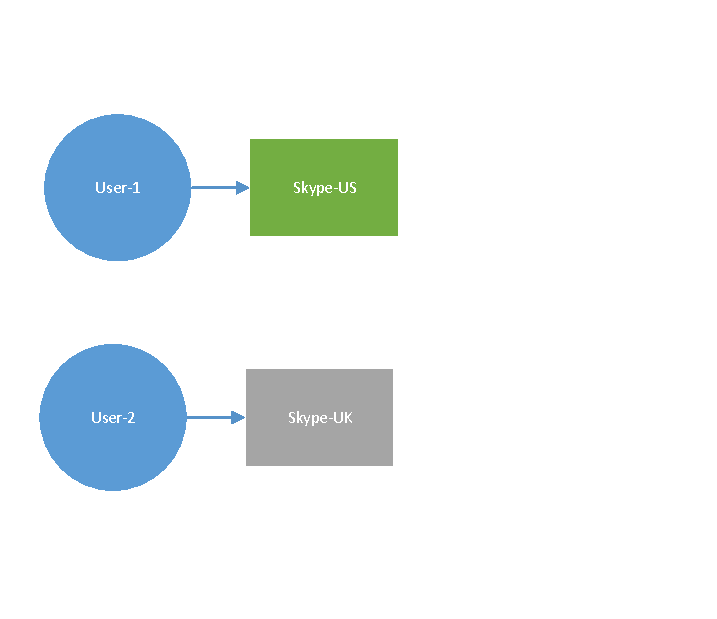
\includegraphics[width=\textwidth]{figures/skype_exampe1.pdf}
	\caption{Without terms layer}
%	\label{fig:skype-no-terms}
\end{subfigure}
\begin{subfigure}[b]{0.49\textwidth}
	\centering
	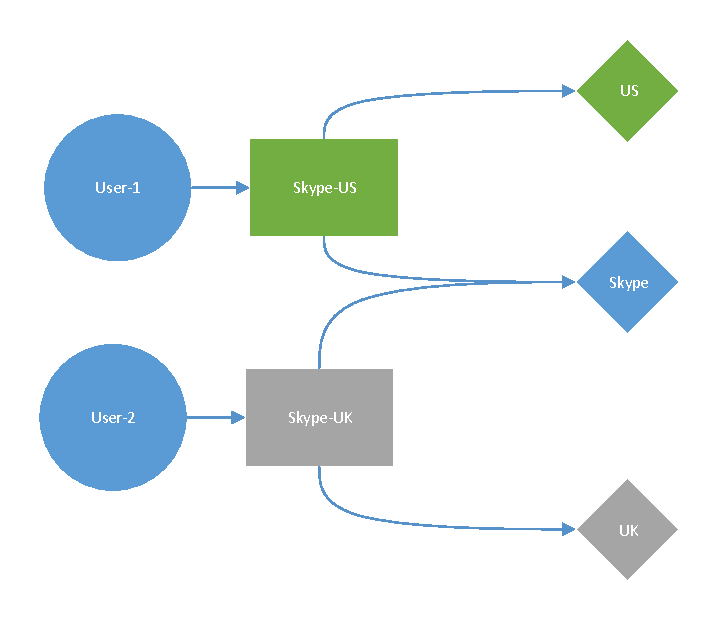
\includegraphics[width=\textwidth]{figures/skype_exampe2.pdf}
	\caption{With terms layer}
%	\label{fig:skype-with-terms}
\end{subfigure}
	\caption{Terms layer example}
	\label{fig:terms_layer}
\end{figure}
  
Figure \ref{fig:sample_graph2} shows another toy graph, demonstrating another aspect of inter-user similarity reflected as connectivity patterns in the graph. This graph includes eight users named shortly as `u-1',`u-2', etc. The eight users are similar in that they share some of the add-ons, `a-1',`a-2', etc. In addition, while {\it add-ons} `a-3' and `a-2' are distinct from each other, these add-on nodes are connected via the common term node `w-skype'. 

We will apply random walks in the graph in order to assess similarity, or relatedness, between users and add-ons.  

\subsection{Data statistics}

The experimental dataset corresponds to a graph that consists of 1,331,814 nodes and 18,552,622
edges. The node and edges types are described at \autoref{tab:node_types}

\begin{table}[H]
\centering
\begin{tabular}{|l|l|}
\hline
\textbf{Type}                                                                & \textbf{Number} \\ \hline
all nodes                                                                    & 1331814         \\ \hline
user nodes                                                                   & 907844          \\ \hline
addon nodes                                                                  & 256458          \\ \hline
term nodes                                                                   & 167512          \\ \hline
high degree nodes (\textgreater500)                                          & 2430            \\ \hline
all edges                                                                    & 18552622        \\ \hline
\begin{tabular}[c]{@{}l@{}}user-addon edge\\   (bi-directional)\end{tabular} & 17612159        \\ \hline
\begin{tabular}[c]{@{}l@{}}addon-term edge\\   (bi-directional)\end{tabular} & 940463          \\ \hline
\end{tabular}
\caption{Nodes and Edges}
\label{tab:node_types}
\end{table}

\begin{figure}[t]
\centering
\begin{subfigure}[b]{0.49\textwidth}
	\centering
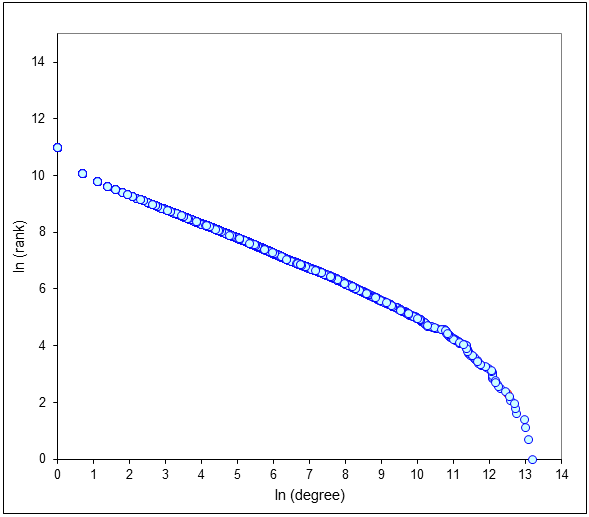
\includegraphics[scale=0.49]{figures/zipf_addon.png} \\
\caption{add-ons} 
\label{fig:power_law_addons}
\end{subfigure}
\begin{subfigure}[b]{0.49\textwidth}
	\centering
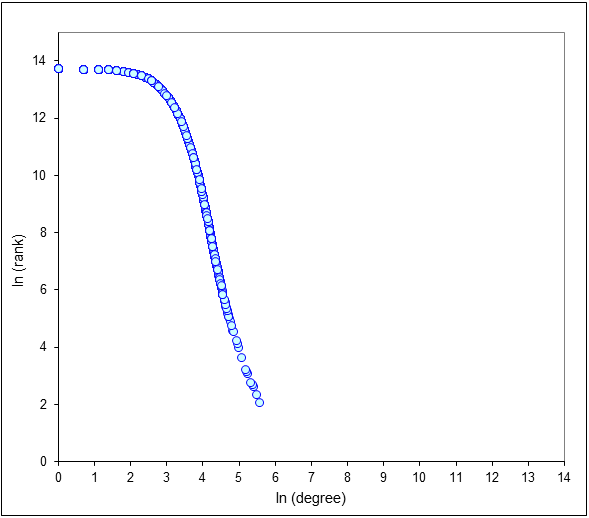
\includegraphics[scale=0.49]{figures/zipf-users.png} \\
\caption{users}
%\label{fig:minlen2noremoveMRR}
\end{subfigure}
	\centering
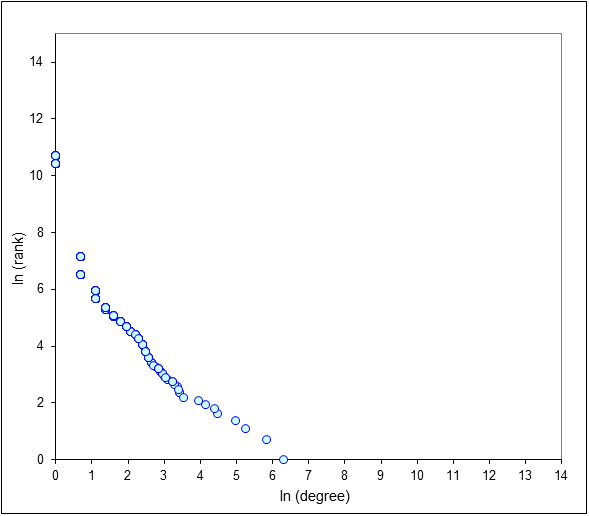
\includegraphics[scale=0.48]{figures/zipf-terms.png} \\
(c) terms \\
\caption{Log-scale rank vs. degree plots of add-ons (a), users (b), and terms (c)}
	\label{fig:zipf}
\end{figure}

\chapter{The missing addon in User ecosystem}
\label{chap:user_ecosystem}

As described in Chapter~\ref{sec:datasets}, we consider authentic user-addon
associations represented as a graph. The graph includes typed nodes
denoting {\it user}, {\it addon} and {\it term} entities, where structured
relations are represented by bi-directional graph edges. In the graph, we expect to observe eco-systems in the form of addons (species) co-existence patterns. 
Supposedly, complimentary addons, or addons installed by ally parties, will be found in the same machines; likewise, rivalry species will not co-exist on one's computing environment. In this chapter, our focus is on alliances that underlie addon distributions, manifested as positive correlations between addons
installed on a user's machines. Concretely, we address the following question:

{\it Given partial information about the addon population at the machine of an individual user--how successfully can we infer the identity of additional species (add-ons) that exist in that environment?}

To the extent that we can predict with high certainty members of a local community, this will support our claim that addon populations are indeed eco-systems and indicate the strength of this phenomena. The merit of the stated
question is that it can be evaluated empirically. We report a
set of link prediction experiments, where the association between random {\it users} and {\it addons} is artificially disconnected, and the `missing links' are then automatically recovered using information about remaining {\it addon} members at the user's environment. Link prediction is manifested in terms of semantic similarity in the graph. To this end, we apply the Personalized
PageRank (PPR) algorithm, a well-studied, scalable, random walk based similarity metric. Using PPR, the thousands of known {\it addons} are ranked by their structured relatedness to the user's environment. We show that the produced rankings included the `missing' addons among the top ranked items, outperforming significantly plausible methods that do not use information about the species that exist in the explored environment, such as ranking addons by their popularity. \iffalse Notably, link prediction is often used a proxy to the task of item {\it recommendation}. \fi

In what follows, we first formalize the task and describe how it is addressed using PPR. We then describe the set of experiments conducted, considering multiple evaluation settings and design choices. The chapter concludes with a discussion of our findings.

\section{Task definition}
\label{sec:task}

Let us denote the graph nodes $G$ as a union of $U,A,T$, the sets of
{\it users}, {\it add-ons} and {\it terms}, respectively. We view this
graph as a global ecosystem. An individual user $u\in U$ is linked in
the graph to its set of add-ons $A(u)$. Let us remove a single item $a_i$
from $A(u)$. User $u$ would be then be associated with a reduced {\it
  addon} set $A(u)'=A(u)-a_i$. We wish to evaluate the extent to which the missing link between $u$ and $a_i$ can be recovered based on the remaining information about the user's environment $A(u)'$ and $G$.

In the rest of this chapter, we will often refer to known set of user \textit{addons}, $A(u)'$, as a {\it query}. Using information retrieval terminology, our goal is to assess the relevancy of possible responses to the query. Specifically, the candidate responses in this case are all {\it addons} that are not known to be associated with the user, i.e., $(A-A(u)')$, where this candidate set includes the target response $a$. As described below, the evaluated methods generate rankings the candidate {\it addons}. Accordingly, performance is evaluated with respect to the rank of the `missing' {\it addon} $a_i$ across multiple instantiated queries. 

\section{Approach}
\label{sec:method}

We employ Personalized PageRank \citep{page1999pagerank} to compute query-specific relevancy scores based on the link structure of the graph. This algorithm models the behavior of a random surfer, who at any given time, chooses
between two possible actions: following a hyperlink to another Webpage, or ``re-setting'', by jumping randomly to one of the pages on the Web. The probability distribution for finding the surfer at any of the graph nodes at time $d$ is computed iteratively, as follows:
\begin{equation}
V_{d+1} = (1-\alpha) [{1 \over N}]_{1 \times N} + \alpha \transition V_d
\label{eq:pagerank}
\end{equation}
\iffalse
\[
\transition = dL + (1-d)[{1 \over N}]_{N \times N}
\]
\fi where the total number of nodes (Webpages) is $N$, and $\transition$
is a transition matrix, modeling the probability that the surfer moves
to page $j$ from page $i$ following a hyperlink. The probability that
the surfer chooses to proceed by following some hyperlink is $\alpha$, and the
probability of the alternative action, re-setting the walk, is ($1-\alpha$) .
\iffalse
$\transition$ distributes a node's probability uniformly among the pages it links
to, i.e.
\begin{equation}
\transition_{ij} = \left}
\begin{array}{lll}
{1 \over |ch(i)|} & \mbox{if there is an edge from $i$ to $j$} \\ 0 &
\mbox{otherwise}
\end{array}
\right.
\label{pagerank_edge_weights}
\end{equation}
where $ch(i)$ is the set of nodes that have an outgoing link from $i$
(the children of $i$).
\fi 
Due to the reset operation, the random walk distribution $V_d$ is guaranteed to
converge to a unique stationary distribution $V^*$. The {\it PageRank score} of node $j$ is defined as its probability in the stationary state $V^*$, giving a measure of document centrality in the network. In general, a node is
assigned a high PageRank score if the sum of the ranks of its
backlinks is high, that is, if it is linked to by other important
Webpages.

The PageRank algorithm described computes universal node importance,
or `centrality' scores, solely based on the network structure, that is,
ignoring user preferences. The {\it Personalized PageRank} variant, as in
\citep{richardson2001intelligent}, biases the random walk model to
generate rankings that reflect user preferences. This bias is modeled by
a small and natural adaptation of the PageRank random walk formula--instead of assuming that the user would reset to any graph node uniformly, reflecting equal interest in all Webpages, it is assumed that only a subset of the graph nodes are of interest to the user. The reset operation is accordingly directed to those nodes, having the random walk scheme modified as follows:
\begin{equation}
V_{d+1} = (1-\alpha) V_u + \alpha \transition V_d
\label{eq:ppr}
\end{equation}
Here, $V_u$ denotes a distribution of interest over the graph nodes,
e.g., nodes that are known to be of interest to user $u$. In general, $V_u$ corresponds to a {\it query} modeled as a distribution over the graph node. The
Personalized PageRank scores, derived from the corresponding stationary state distribution, reflect structural similarity, or relevancy, of the graph nodes with respect to the query. 

It has been shown that the Personalized PageRank score for a target node $z$ and a query node $x$ equals a summation over all of the connecting paths between $x$ and $z$ (including cyclic paths, and paths that cross $z$ multiple times), where paths are weighted by their probability \citep{jeh2003scaling},\citep{fogaras2004towards}. In words, the graph walk
distributes probability mass from the start distribution over nodes through edges in the graph---incidentally accumulating evidence of similarity over multiple connecting paths. Due to the reset probability $(1- \alpha)$, the paths between $x$ and a destination node $z$ are weighted exponentially lower as their length
increases. This implies that graph nodes that are connected to the query nodes over shorter connecting paths, as well as over multiple connecting paths, are considered more important with respect to $V_u$. Fortunately, the computation for a multi-node query is no more difficult than for a single-node query due to the
\textit{Linearity Theorem} \citep{jeh2003scaling}, as the Personalized
PageRank vector for a multi-node query is a simple linear combination
of the individual PPV for each node in the query.

\iffalse
The graph walk process (and accordingly, the similarity measure
generated) is determined by the graph's topology.\footnote{The reset
probability $\gamma$ has negligible effect on the generated rankings;
see a related discussion in Section \ref{sec:graph_walk_parameters}.}
In addition, the walk on the graph is controlled by a set of edge
weight parameters $\Theta$. This means that throughout the graph,
edges of type $\ell$ are assigned a typical edge weight $\theta_{\ell}
\in \Theta$. Let $L_{xy}$ denote the set of edge types of the outgoing
edges from $x$ to $y$. The probability of reaching node $y$ from node
$x$ over a single time step (corresponding to the transition
probability $\transition_{x,y}$) is defined as:

\begin{equation}
Pr(\edge{x}{}{y}) = 
{\sum_{\ell \in L_{xy}}\theta_{\ell} 
\over 
\sum_{y' \in ch(x)}\sum_{\ell' \in L_{xy'}}\theta_{\ell'}}
\label{eq:transition1}
\end{equation} 
where $ch(x)$ denotes the set of children of $x$ (the nodes reachable
from $x$ in one time step). That is, the probability of reaching node
$y$ from $x$ is defined as the proportion of total edge weights from
$x$ to $y$ out of the total outgoing weight from the parent
$x$.\footnote{The PageRank scheme given in Formula
  \ref{pagerank_edge_weights} is a special case of Equation
  \ref{eq:transition1}, where the graph includes a single edge type,
  and weights are distributed uniformly.} The graph edge weights
$\Theta$ can be set uniformly; randomly; manually, according to prior
beliefs; or using a learning procedure. The edge weights $\Theta$
provide another mechanism for affecting the probability flow in the
graph.
\fi


\iffalse In this thesis the goal of biasing the PageRank with the
teleportation vector is to personalize the user addons of choice
results.  Instead of looking at a “random surfer” on the web, the
non-web PageRank models a random walk on the graph. The behavior of
the walk is the same as the random surfer: with probability $\alpha$
the walk continues along an edge of the graph and with probability
1-$\alpha$ the walk jumps to a random node in the graph. Personalized
PageRank is an important extension of PageRank model, in which the
surfer does not randomly restart browsing anywhere on the web after
choosing not to follow a link. Rather, the surfer in this new model
restarts at one of only a few pages. If the pages relate to one
person, then the resulting PageRank vector is called a personalized
PageRank vector. If the pages are topically related, then the vector
may be called a topic-specific PageRank vector.  \fi

\iffalse
Personalized PageRank is an extension of the famous PageRank algorithm
\cite{page1999pagerank}, both of which are based on a random surfer
model. To understand Personalized PageRank, we first review the
original PageRank briefly. A random surfer starts at any node on the
graph. At each step, with a probability of 1\−$\alpha$ the surfer moves
to a neighboring node randomly, and with a probability of $\alpha$ he
teleports to a random node on the graph. This process is repeated
until the walk converges to a steady-state. The stationary probability
of the surfer at each node is taken as the score of the node. However,
this form of score is purely based on the static link structure,
indicating the overall popularity of each node on the graph, without
tailoring to a specific query node.\\ In contrast, Personalized
PageRank enables query-sensitive ranking, in the sense that we can
specify a query node to obtain a “personalized” ranking
accordingly. It is based on the same random surfer model of the
original PageRank, except when the surfer teleports, he always prefers
the query node \textit{q}. Specifically, at each step, with
probability $\alpha$ the surfer teleports to \textit{q} instead of a
random node, thus visiting the neighborhood of \textit{q} more
frequently.  Thus, the stationary distribution, called a Personalized
PageRank Vector (PPV), is biased towards \textit{q} and its
neighborhood, which can be interpreted as a popularity or relevance
metric specific to \textit{q}.  More generally, a query \textit{q} can
comprise multiple nodes on the graph, such that in the teleportation
the surfer can jump to any node in \textit{q}. Fortunately, the
computation for a multi-node query is no more difficult than for a
single-node query due to the \textit{Linearity Theorem}
\citep{jeh2003scaling}, as the PPV a multi-node query is a simple
linear combination of the individual PPV each node in the query.

A personalized PageRank vector, also known as a random-walk with
restart (RWR), is the stationary distribution of a random walk that,
with probability $\alpha$ follows a step of a random walk and with
probability (1−$\alpha$) jumps back to a seed node.  If there are
multiple seed nodes, then the choice is usually uniformly random. The
set of these seeds is called personalized PageRank Vector (PPV).  
\fi

\iffalse 
with users and looking for their personal
preferences in browsers extensions, we are also interested in Company
based addons propagation in users network. All our dataset was
transformed to undirected graph, where user nodes are connected to
addon nodes according to their relationship in the original dataset,
e.g. each user node has an edge connected to addon node if this user
has this addon installed in its ecosystem. Since our goal is to
determine/predict a missing addon in user ecosystem, the seed nodes
for the personalization vector would be the specific user addons, our
hypothesis is that a higher the PageRank score suggests a higher
relevance of an addon to the specific user. We would run multiple
experiments to show the correctness of our hypothesis.  
\fi

\iffalse
\subsection{Support Vector machine}
First we have tried running analysis on our data using SVM. We were
trying to classify users that are staying long in user ecosystem and
those that churn immediately, lately this would turn to Clash
prediction.\\ We have defined training data as follows - positive
examples are the users that have stayed at the system more than three
days and others are negative example. We have used a popular libSVM
tool to run the analysis.\\ The training very long time and gave no
results, trying to run SVM with another kernel did not help either -
and every run took a few days to finish. Then we've decided to find
another way to represent our data.
\subsection{GraphChi}
\subsection{iGraph}
\fi

\subsection{Predicting the missing add-on using PPR}

The question that we wish to answer in this research is `given
a set of {\it add-ons}, which are known to co-exist on the machine of
some user, what other {\it add-ons} are most likely to be linked to
that user?'. This question is addressed by means of structural
similarity in the graph. Formally, we assign $V_u$ to be uniform over $A(u)'$, that is, the re-set probability to each of the nodes representing {\it add-on} $a\in A'$ is set to ${1 \over \mid A' \mid}$, and is zero otherwise. The constructed transition matrix $\transition$ assign equal importance to all of
the graph edges. That is, the transition probability from node $i$ to
a linked node $j$ is defined as: $_{ij}={1 \over \mid N_i \mid}$,
where $N_i$ is the set of nodes linked over an outgoing edge from $i$. For example, suppose that node $i$ is linked to two {\it term} nodes and five {\it user} nodes; then, the probability of reaching any of these nodes using the transition operation equals ${1\over 7}$. In general, it is possible to assign varying edge weights, either using parametric weights according to edge types, or deriving such weights from local edge properties. Recent works have also considered learning a selective set of meaningful paths in the graph that link query with target nodes \citep{minkov2010improving,lao2010relational} We leave the exploration of learned random walk measures to future work. 

The computed Personalized Pagerank vector assigns scores to all of the
graph nodes. We rank the graph nodes of type {\it addon} by their PPR score. It is conjectured that the `missing add-on' will be included among the top-ranked items in the list, due to high structural coherence with the set of addons that comprise the query. Concretely, the probability mass assigned to the query nodes is expected to flow over multiple path types, reflecting the following main types of structural similarity:
\begin{itemize}
\item {\it User-based similarity}: A dominant short path that
  directly leads to related add-ons is {\it add-on} $\Rightarrow$ {\it user}
   $\Rightarrow$ {\it add-on}. This path links each of the query addons
  with other users that have the same addon installed on their
  machine. Walking away from these {\it user} nodes to their associated
  {\it addons} should highly weight addons that frequently
  co-occur with the input addon on the same machines. As the query consists of multiple {\it addon} nodes, the resultant PPR scores are expected to prioritize {\it addons} that co-exist on users' machines with multiple input addons.   
\item {\it Term-based similarity}: As demonstrated before
  (Sec. \autoref{sec:graph_representation}), the name and descriptions of addon
  instances exhibit lexical variations. For example, similar addons may vary with respect to the software's version number. The constructed graph links each {\it addon} node with the {\it terms} that it contains. Thus, co-reference resolution can take place via the path {\it addon}
  $\Rightarrow$ {\it term} $\Rightarrow$ {\it addon}. Also here, the graph-based similarity metric favors {\it addons} pairs that connected over multiple {\it terms}. 
\end{itemize}

The stationary distribution of the random walk process manifests long-range relationships in the graph, consisting of various concatenations of the paths listed. We therefore expect that co-occurrence of coreferent {\it addons} will be also reflected in the random walk results.


\section{Experimental methodology}

We derive labeled queries from our corpus for evaluation purposes.  Each query corresponds to a randomly selected user $u$. Having selected the user node $u$, we further randomly select one of its linked {\it addons} $a$. The selected addon is eliminated artificially from the user's `profile', having the link between the nodes denoting $u$ and $a$ disconnected in the graph. In
the experiments, we evaluate the extent to which the missing link can
be recovered. 

The process of generating an individual labeled example is formally outlined in Figure \ref{fig:example-gen}. Obviously, the sampled users are required to have at least two addons installed on their machine--otherwise, the query vector would be left empty, once detaching the target addon from the user node for testing purposes. 

\begin{figure}
\begin{enumerate}[(a)]
\begin{small}
\item Pick uniformly at random a {\it user} node $u$ from the graph.
\item Find the set of {\it add-on} nodes linked to $u$, $A_u$.
  all its addon nodes.
\item Pick uniformly at random an addon node $a$ from the set $A_u$. 
\item Disconnect the link between nodes $a$ and $u$ in the
  graph. Since the only connection between a user node and the addon
  node is the edge between them, by simply deleting this edge we are
  removing this addon from user profile.
\item Let the query $V_u$ be a uniform distribution over $\{A_u-a\}$,
  and the correct answer to the query be $a$. 
\end{small}
\end{enumerate}
\caption{The process of generating an individual labeled example}
\label{fig:example-gen}
\end{figure}

Once disconnected from the user node, there should be no selection bias towards the target addon $a$ compared with the other addon nodes in the graph. As discussed above, PPR's ranking scheme should discover association between the removed add-on and the addons still associated with the user. Naturally, the addons included in the query are assigned high relevancy scores by query-sensitive algorithms like PPR. The query addons are therefore discarded from the evaluated ranked list. 

For example, suppose that we uniformly at random choose a user that has five addons -skypeclicktocall.dll, windowslivelogin.dll, skypeieplugin.dll, linkverifier.dll and googletoolbar\_32.dll. Let us sample the googletoolbar\_32.dll as the target addon. The remaining four addons form the query vector. After executing the PPR, the four query nodes are removed from the ranked list.

\subsection{Evaluation measures}

\iffalse Now, like in \autoref{sec:PPR_addons_method},
when we are predicting the missing add-on, we are looking at the
addons ranking list (the ranking is according to PageRank scores) and
check the Recall@K. This measure seems to give similar results as the
Popularity baseline.\fi

\iffalse Since, lets say it is ranked in 8th position, not
taking into account the ranking position of the original user addons,
then we could recommend to user top ten scored addons and with high
probability user will find a usefull addon between this
ten.\\ \textcolor{green}{\textit{Sela: Example:}}
\textcolor{green}{\textit{Einat:How was evaluation conducted? cross
    validation.. using MAP meausre(?)  (can include a description of
    MAP as an appendix)}} \fi

We experiment in this work with PPR and alternative methods. All methods generate scores, which are processed into output ranked lists of addons. Accordingly, we assess performance using a set of metrics designed for the evaluation of ranked lists. Note that in our settings, there is a single known `correct' answer. The various metrics assess the extent to which each method places the relevant response at the top of the ranked list, on average across all queries. A short description of the evaluation measures follows.

\paragraph{Recall at rank k}
This is the fraction of queries, for which the relevant response is included among the top $k$ ranks (see also \citep{minkov2010improving}). The non-interpolated recall at rank k of a given ranked list is defined to be 0 for each rank $k = 0, ..., k_{i−1}$, where $k_i$ is the rank that holds the single correct entry, and 1 for ranks $k\geq k_i$. The (mean) recall at rank $k$ averages the recall
scores at each rank $k$ across the rankings of multiple queries. Thus, mean recall is in the range [0,1] at each rank $k$. For example, recall at rank
3= 0.7, means that in 70\% of the queries, the correct answer appears among the
top 3 ranks of the retrieved lists.

\paragraph{Mean Reciprocal Rank (MRR)}

The mean reciprocal rank metric \citep{voorhees1999trec} considers the position of the first correct answer in the ranked list.  As formalized in Eq.~\eqref{eq:mrr}, the non-interpolated reciprocal rank is the inverse of the position of the correct item (addon) in the ranked set for a given query; the MRR score is the mean reciprocal rank across all of the queries. Unlike the recall-at-rank-k measure, which disregards the results below rank $k$ for evaluation purposes, MRR is based on the full list of ranked items. such measures (once extended to consider multiple correct answers) are especially informative in assessing recommendation quality in domains that target a small set of valuable items, such as friends recommendation in social
networks \citep{chen2006less}. 
\begin{equation}
 MRR = \frac{1}{Q} \times \displaystyle\sum\limits_{q=1}^{Q} \frac{1}{rank_q)}
\label{eq:mrr}
\end{equation}

For example, suppose that the removed addon is placed at rank 20 in response to an individual query by the evaluated method. This result will not contribute to mean Recall@10 score; it will contribute however to Recall@20 score (or mean recall at any rank lower than 20). The contribution of this result to MRR is ${1 \over 20}=.05$.

\section{Experiments}
\label{sec:experiments}

We use Personalized PageRank to rank {\it add-on} nodes in
the graph by their structural similarity to the user profile, or {\it
  query}. The generated rankings using this approach may be affected
by design choices concerning the graph structure and the random walk scheme. This section first provides details regarding the implementation of PPR, and provides details about baseline methods that we compare against. It then discusses aspects concerning the graph design that are evaluated in this work.

\subsection{Methods}
\label{sec:methods}

In the experiments, we make use of a fast and memory-efficient implementation of Personalized PageRank included in {\it igraph} \citep{igraph}, a software library optimized for the processing large-scale graphs. {\it iGraph} uses internally the ARPACK package, a numerical software library written in FORTRAN 77, for solving large scale eigenvalue problems (often used in analyzing large social networks, e.g., \citep{ting2004minig}). ARPACK applies an implicitly restarted Arnoldi method to calculate the random walk scores. \iffalse igraph expects as an adjacency list of numeric
vertices. We have created a unique number for each node and store the
mapping to an actual node name in a separate file.\fi The computation of PPR scores is highly efficient, as the whole graph is loaded into memory. \iffalse, we had to be very careful with memory
management (every very small leak would cause a serious global memory
leak).\fi We ran the experiment using a standard PC machine using a a 64bit version of igraph, which was adapted for our needs and bug fixes were applied. On average, running a batch of 1,000 queries required a few hours. In the experiments, we set the teleport probability parameter $\alpha=0.85$ following previous works \citep{boldi2005totalrank}. In general, due to the exponential decay over distance from the query nodes implied by PPR's random walk formula, the teleport probability value has negligible effect on the produced rankings.

We further evaluate two non-personalized alternative ranking methods: ranking {\it add-ons} by `popularity', as well as based on their PageRank scores. 

\subsubsection{Popularity baseline} 

A simple approach for predicting the `missing' add-on would be to rank the {\it add-on} items by their popularity, determined by the total number of users associated with each add-on in the corpus. Using this approach, the response to all queries is fixed, having the output list ranked according to the popularity criterion. In other words, since the algorithm performs no personalization, all users are presented with the same
add-on list. Despite its simplicity, the popularity algorithm can perform reasonably well when item popularity follows a power law distribution. An advantage of this algorithm is that it is non-parametric and scalable; item scores may thus be computed efficiently for corpora that contain hundreds of thousands of users and tens of millions of items by means of database querying. 

\subsubsection{PageRank baseline} 

For each addon we have calculated its PageRank score given the underlying graph. The PageRank scores assigned to the graph nodes reflect their structural centrality in the graph. We are interested in comparing PPR performance with this non-personalized version of the random walk algorithm.

Both baselines were implemented using {\it igraph}. \iffalse were implemented in a high performance, parallel
or distributed environment. We chose to use igraph \citep{igraph}, a
high-performance, parallel machine learning framework. \fi

\subsection{Graph design choices}
\label{sec:design}

The proposed graph schema is simple and natural in the sense that it directly represents the relational structure of the source information. We discuss in this section a set of considerations involved in fine tuning of the graph design. The impact of the design options detailed below is evaluated empirically.  

\subsubsection{Pruning of high-degree nodes} 

Several previous works have indicated that high-degree nodes in the graph have negative impact on the PPR similarity measure \citep{tong2006center}. High density of the transition matrix results in increased computation cost of the random walk process. Further, the random walk process exhibits some bias in favor of high degree nodes. According to \citep{sarkar2010fast}, removing high degree nodes should only result in only a small approximation error, see also \autoref{sec:ppr_high_degree}. Indeed, the graph walk schema implies that the probability mass assigned to high-degree nodes be distributed among a large variety of neighboring nodes in the random walk process, thus having little impact on the final rankings. At the same time, high-degree nodes receive a large number of contributions from their neighbors, and are therefore highly-ranked. Removing these nodes from the graph will increase the `visibility' of lower-degree nodes. Finally, we wish that the Personalized PageRank scores reflect node relevancy with respect to the input query vector, representing the user's ecosystem. Influential high degree nodes may weaken the association with the query seeds.

We report experimental results using the full graph, as well as using a graph variant, in which high-degree nodes are removed. We define high-degree nodes in this work as nodes for which the out-degree is equal or higher than 500. As shown in Figure~\ref{fig:zipf}, only a fraction of the most popular {\it addons} have a greater out-degree and are pruned in this fashion. Note that given a graph variant in which these `popular' nodes have been removed, the sampled queries no long include popular {\it addons}, but rather contain only lower-frequency addons, which are more challenging to predict. We believe that this latter configuration is of special interest for recommendation purposes; if one wishes to recommend addons to users, focusing on non-trivial items can be highly beneficial.

\subsubsection{Term modeling}

The modeling of {\it term} nodes is desirable as it establishes links between related addons, e.g., add-ons with the same name but with different version numbers. Specifically, version numbers are included either as a suffix to the add-on name, or as a directory name part of the path string. Splitting the add-on names into tokens and linking the respective {\it add-on} and {\it term} nodes should maintain connectivity between multiple version of the same {\it add-on}, where consequently this should improve the graph relatedness measure. On the other hand, it is possible that linking {\it add-ons} over shared {\it terms} will result in a topical drift. Assuming, for example, that the user is known to have an {\it add-on} that has to do with video streaming and has the term `video' as part of its name; other {\it add-ons} reached by traversing a term-hopping path may have similar functionality. In this fashion, given the user's query, the ranked list of results may include {\it add-ons} that are similar or alternative to the {\it add-ons} that are known to be installed at the target user, pushing downwards in the rankings those {\it add-ons} that are complimentary to the users eco-system. Experimental results using graphs with and without {\it term} nodes shows that overall, term modeling has positive effect in predicting the `missing' add-on.

\subsubsection{Specificity of path information} 

Addon names often include full file-system path information, e.g., \\
`C:/Program Files (x86)/Skype/skype1.dll'.In our main experiments we remove path prefixes \\
(like `C://Program Files (x86)/skype') for several reasons. First, we wish to represent every unique add-on as a distinct node in the graph. Including path details in the add-on name will result in multiple copies of the same add-on merely due to differences in local installation sites. Such redundancy may have negative effect on the produced  graph-based node relatedness metric, as well as bias the evaluation. 
Suppose that the target add-on is included in the answer list with a path prefix that is different from the one used in the target user's machine; if we kept the path, then it would be considered as incorrect answer, while removing the path should help us to identify it as the same add-on. In addition, Supposedly, it can be harmful to link add-ons to common {\it terms} associated with path information (e.g., `program'; `files'; `x86'). Such links may connect add-ons due to machine configurations that are meaningless semantically (although, the term `skype' would be potentially useful in this case.)


\section{Results}
\label{sec:user_main_results}

\iffalse
1) `default' scenario:

Use the graph with popular nodes. Compare these variants:
- Popularity baseline
- PageRank baseline
- PPR, users+addons, without paths
- PPR, users+addons+terms, without paths

Show results for 4X1000. MMR / recall@k.

Main findings: we outperform popularity; also, representation of terms helps.

2) Focus on lower-degree add-ons:

- The scores are approximately correct when high-degree nodes are removed.
- Reduces computational costs.
- Low-degree nodes are interesting, but popularity and PR methods only include them at the bottom of the list.

2A) Include analysis of degree distribution: 
-- show number of nodes by degree, log-scale. (look for example graphs of Zipf's law).
-- Same, for add-ons.
-- Same, for terms.
-- Same, for users. (do not use log-scale if it doesn't make sense, as in this case.)

2B) Use the graph without high-degree nodes. (Re-compute the pop. and PR baselines.)
- Popularity baseline
- PageRank baseline
- PPR, users+addons, without paths
- PPR, users+addons+terms, without paths

SENSITIVITY:

3) Impact of paths:

What happens if we include the full path?

Detail number of add-ons before and after filtering. 

- Full graph, users+addons+terms
- High-degree removed, users+addons+terms

- Full graph, users+addons
- High-degree removed, users+addons

4) Sensitivity to # of add-ons per user: (>=2, >=3, ..)

Can show results of multiple configurations as curves on the same graph.
\fi

\paragraph{Main results}

Throughout this section, we report results using query sets that include $Q=1000$ labeled examples of randomly sampled user-addon pairs per individial experiment. Each experiment was repeated using four sets of queries (4$\times$1000). Wherever possible, we report mean results alongside standard deviation.  

Let us first consider the general scenario, in which the underlying graph contains all of the {\it add-ons}, including the most prevalent ones. Figure~\ref{fig:main} shows recall-at-k performance using PPR, comparing it against ranking-by-popularity and PageRank rankings. Full results, including standard deviation figures and MRR results are detailed in Table~\ref{tab:full}.
As shown in Figure~\ref{fig:main}(a), PPR rankings yield consistently preferable performance to the alternative methods. Recall-at-rank-10 using PPR is as high as .354, reaching recall of .660 and .801 at the top 50 and top 100 ranks, respectively. Compared with the non-personalized popularity-based ranking, recall-at-10 results improve at a high rate of 45.7\% using PPR (.354 vs. .243). Improvement rates at rank-50 and rank-100 measure 18.9\% and 12.7\%, respectively. These results indicate that PPR excels at recovering the missing add-on in general, and is more successful in ranking it at the top 10 ranks.  Interestingly, performance using the popularity- and PageRank-based rankings is nearly identical. This result is not very surprising as the most popular {\it add-ons} are likely to be prominent in terms of graph centrality. 

\begin{figure}[t]
\centering
%\begin{subfigure}[b]{0.49\textwidth}
	\centering
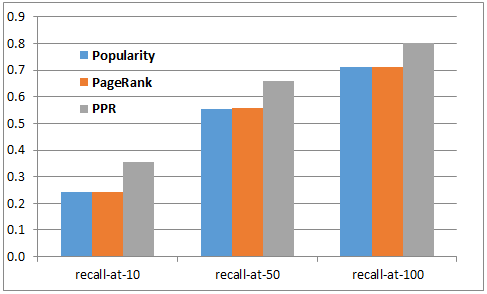
\includegraphics[scale=0.8]{figures/pop-final.png} \\
(a) \\
%\caption{Recall@K}
%\label{fig:minlen2remove500Recall}
%\end{subfigure}
%\begin{subfigure}[b]{0.49\textwidth}
	\centering
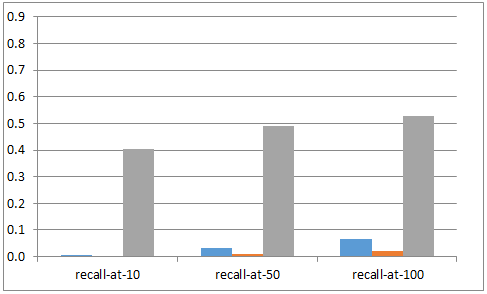
\includegraphics[scale=0.8]{figures/sans-popular-final.png} \\
(b) \\
%\caption{MRR}
%\label{fig:minlen2remove500MRR}
%\end{subfigure}
	\caption{Main results: recall at top ranks for the full graph (a), and a graph excluding the most popular add-ons (b)}
	\label{fig:main}
\end{figure}


\begin{table}[p]
\centering
\caption{Standard deviation and Standard error of the Mean}
\label{tab:full}
\begin{tabular}{llcccc} \hline
	& & Recall-at-10 & Recall-at-50 & Recall-at-100 & MRR	 \\
\hline
\multicolumn{6}{c}{FULL} \\
\hline
& POP & 0.243 (0.007) & 0.555 (0.017) & 0.711 (0.012) & 0.104 (0.004) \\
& PR & 	0.243 (0.007) & 0.559 (0.016) & 0.711 (0.012) & 0.104 (0.004) \\
& PPR	& \textbf{0.354}	(0.011) & 0.660	(0.009) & 0.801 (0.004) & \textbf{0.151}	(0.006) \\
\hline
No terms & POP & 0.240 (0.009) & 0.553 (0.012) & 0.719 (0.007) & 0.101 (0.005) \\
& PR & 0.240 (0.009) & 0.563 (0.014) & 0.719 (0.007) & 0.101 (0.005) \\
& PPR	& 0.350	(0.014) & \textbf{0.665}	(0.008) & \textbf{0.809}	(0.014) & 0.146	(0.008) \\
\hline
Full path & POP & 0.065 (0.005) & 0.177 (0.010) & 0.224 (0.010) & 0.023 (0.004) \\
& PR & 0.185 (0.013) & 0.409 (0.016) & 0.538 (0.012) & 0.079 (0.010) \\
& PPR	& 0.294	(0.017) & 0.592	(0.015) & 0.708	(0.010) & 0.150	(0.008) \\
\hline
\multicolumn{6}{c}{SANS POPULAR NODES} \\
\hline
 & POP & 	0.006 (0.004) & 0.034 (0.009) & 0.065 (0.009) & 0.004 (0.001) \\
 & PR	& 0.001	(0.000) & 0.009	(0.009) & 0.022	(0.003) & 0.001	(0.000) \\
& PPR	& 0.405	(0.007) & 0.491 (0.007) & 0.527	(0.004) & 0.320	(0.005) \\
\hline
No terms & POP & 	0.000 (0.000) & 0.000 (0.000) & 0.000 (0.000) & 0.000 (0.000) \\
& PR & 	0.001 (0.002) & 0.012 (0.007) & 0.027 (0.002) & 0.001 (0.000) \\
& PPR & 	0.401 (0.027) & 0.483 (0.027) & 0.521 (0.022) & 0.322 (0.027) \\
\hline
Full path & POP & 	0.004 (0.003) & 0.019 (0.006) & 0.033 (0.007) & 0.003 (0.001) \\
& PR & 	0.032 (0.010) & 0.033 (0.010) & 0.034 (0.010) & 0.001 (0.000) \\
& PPR	& \textbf{0.496}	(0.017) & \textbf{0.575}	(0.022) & \textbf{0.602}	(0.016) & \textbf{0.415}	(0.020) \\
\hline
\end{tabular}
\end{table}

Next, we discuss our results using the graph variant, in which highly-connected addons have been removed (Sec.~\ref{sec:design}). This scenario is more challenging, as the queried disassociated {\it add-ons} are not highly-frequent in the global population. The results of this experiment are shown in Figure~\ref{fig:main}(b) and Table~\ref{tab:full}. As one might expect, performance of the popularity-based baseline plummet in this case; recall-at-10 is nearly zero (.006) and recall-at-100 is also very low (.065). Using PageRank gives comparable (and slightly lower) results compared with the popularity rankings. In contrast, PPR maintains its effectiveness: recall-at-rank-10 is .405 using PPR, reaching .491 and .527 at ranks 50 and 100, respectively. While recovering links to non-popular add-ons may be harder, recall performance at the top 10 ranks is in fact better using PPR in this scenario (.405 vs. .354). This indicates that popular nodes occupying the top ranks `push' relevant yet less popular answer nodes to lower positions of the ranked list.  

Overall, we conclude from these experiments that there indeed exists high structural semantic association between the add-ons installed on one's machine, to the extent that it is possible to predict one of these add-ons if removed randomly. Personalized PageRank is shown to provide an effective mechanism for this task, as it evaluates nodes by their structural joint similarity to the set of add-ons present at the specified environment. 

\subsubsection{Impact of term modeling}

As discusses earlier, we include {\it terms} in the graph, so as to model term-based lexical similarity between co-referent (or generally similar) add-on descriptions. We are thus interested in evaluating the contribution of term modeling to our task. Table~\ref{tab:full} shows the results of all methods using the same underlying graph, where {\it term} nodes have been removed. The resulting graph is therefore bi-partite, including {\it user} and {\it addon} nodes only, connected over bi-directional {\it has-addon} edges. Again, we evaluate two graph configurations--with and without the high-degree {\it addon} nodes. According to the reported results, term modeling has positive yet low impact on the produced rankings. Overall, MRR performance is slightly higher with terms included when popular nodes are present (.151 vs. .146), partly due to better recall  performance at the top 10 ranks (.354 vs. .350). Using the graph without the popular nodes, recall performance at the top 10 ranks also improves (.405 vs. .401), and recall-at-rank-50 and recall-at-rank-100 show similar improvement; MRR is roughly comparable in this case (.320 vs. .322). Overall, while positive, the contribution of {\it term} modeling is modest. 

We were interested in investigating the reasons for the relatively low impact of {\it term} nodes in the graph. In another experiment we used a graph variant that included {\it addons} and {\it term} nodes only (i.e., without {\it users}); ranking performance using this graph variant was poor. We suggest the following explanation for these results. In the graph, {\it addon} nodes are typically connected to a large number of {\it user} nodes, and only to a very few {\it term} nodes. To illustrate this, consider some arbitrary addon for which a short description is available. This {\it addon} node will link to a few (roughly, three) {\it term} nodes, and a medium user set neighborhood (roughly, 200) {\it user} nodes. Since the random walk distributes probability mass uniformly over all neighbors of a source node, the total probability flow through the {\it term} nodes is relatively small. Assigning higher weight to links leading to {\it term} nodes (see~\citep{minkov2010improving}) will increase their traversal probability and increase their impact. We leave the exploration of this possibility for future work.

\subsubsection{Sensitivity to path information}

Table~\ref{tab:full} further shows experimental results using graph variants in which {\it addons} were represented by the full path. Again, both the graph variants, with and without high-degree nodes, are evaluated. We observe that when path information is present in the full graph, recall performance using PPR is somewhat degraded (e.g., recall-at-rank-10 is reduced from .354 by 17\% to .294). In contrast, when high-degree nodes are removed from the graph, PPR performance is improved when path information is modeled (recall-at-rank-10 increases by 22.5\% from .405 to .496). We suspected that this improvement was due to contribution of {\it terms} extracted from the path, leading the algorithm to favor {\it addons} based on path configuration information--such an association would be technical rather than semantic. However, repeating the experiment having the  {\it term} nodes removed from the graph still yielded impressive performance gains, compared with the graph with no path information (e.g., recall-at-10 measured at .478). We conjecture that path information is in fact {\it meaningful} for the task at hand. In particular, paths may differ by language, where it is likely that eco-systems vary geographically. Or, the path on which addons are installed may indicate by itself on sub-groups in the population (e.g., advanced users who use certain operating systems, and vice versa). 
When there is little variance among users, better statistics is obtained without path information; this may be the case in the full graph scenario, where most queries correspond to highly frequent nodes, possibly sampled from one dominant cluster (say, U.S. users, who use standard operating system). 

Finally, the performance of the popularity-based approach plummets in this setting (recall-at-rank-10 diminished by 73.3\% from .243 to .0065). PageRank's performance is affected to a lesser extent (recall-at-rank-10 reduced by 23.9\% from .243 to .185). These trends are in line with our observation, by which path information impairs the statistical information, upon which these methods base their predictions.

\iffalse
\begin{figure}[t]
\centering
\begin{subfigure}[b]{0.49\textwidth}
	\centering
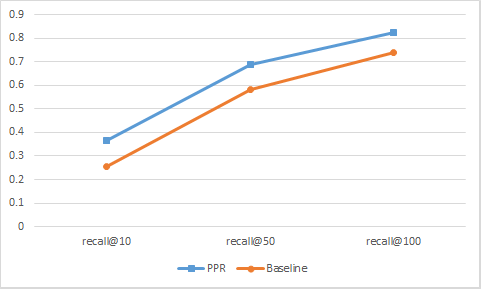
\includegraphics[scale=0.49]{figures/minlen2noremove.png}
\caption{Recall@K}
\label{fig:minlen2noremoveRecall}
\end{subfigure}
\begin{subfigure}[b]{0.49\textwidth}
	\centering
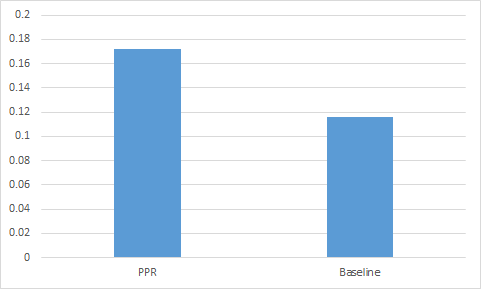
\includegraphics[scale=0.49]{figures/minlen2noremoveMRR.png}
\caption{MRR}
\label{fig:minlen2noremoveMRR}
\end{subfigure}
\caption{Graph without paths with popular nodes}
	\label{fig:minlen2noremove}
\end{figure}
\fi



\iffalse
\begin{figure}[t]
\centering
\begin{subfigure}[b]{0.49\textwidth}
	\centering
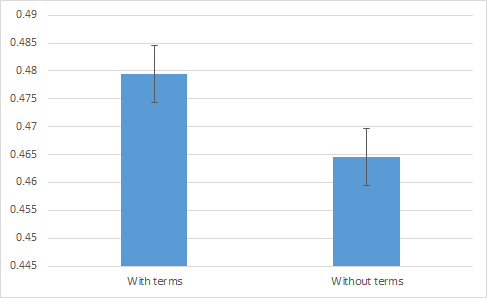
\includegraphics[scale=0.49]{figures/5addonswithoutTermsComp.png}
\caption{With/without term nodes with paths without popular nodes}
\label{fig:with_without_terms5}
\end{subfigure}
\begin{subfigure}[b]{0.49\textwidth}
	\centering
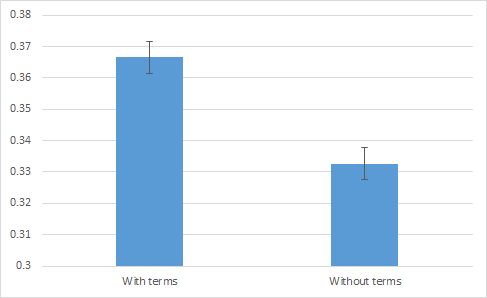
\includegraphics[scale=0.49]{figures/2addonswithoutTermsComp.png}
\caption{With/without term nodes without paths with popular nodes}
\label{fig:with_without_terms2}
\end{subfigure}
\caption{Comparing graph with/without addon paths}
	\label{fig:with_without_terms}
\end{figure}
\fi


\iffalse
\begin{figure}[t]
\centering
\begin{subfigure}[b]{0.49\textwidth}
	\centering
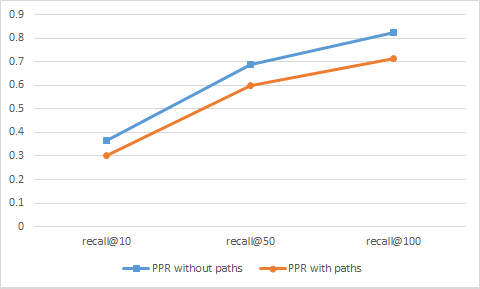
\includegraphics[scale=0.49]{figures/minlen2noremoveCompPaths.png}
\caption{With/without addon paths with popular nodes}
\label{fig:with_without_paths_noremove}
\end{subfigure}
\begin{subfigure}[b]{0.49\textwidth}
	\centering
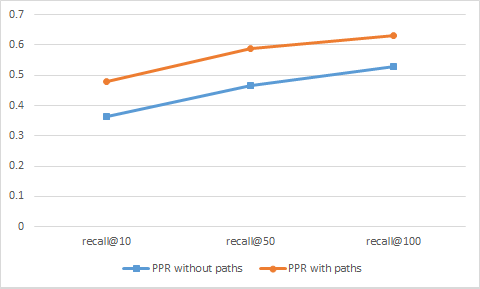
\includegraphics[scale=0.49]{figures/minlen5remove500CompPaths.png}
\caption{With/without addon paths without popular nodes}
\label{fig:with_without_paths_remove500}
\end{subfigure}
\caption{Comparing graph with/without addon paths}
	\label{fig:with_without_paths}
\end{figure}
\fi

\paragraph{Sensitivity to environment size}

As mentioned earlier, we select users that have at least two add-ons installed on their machines. Figure~\ref{fig:addonsNumberGraph} shows recall performance at the top ranks using PPR per different sampled populations: users who have at least $N$ addons installed, having $N=2,4,5,10,15,20$. It is shown that recall levels decrease as the number of addons known to be installed at the user's machine grows. We believe that as more species co-exist on one machine, higher heterogeneity is introduced to the system, where sub-groups of addons cluster together. PPR may find addons that are semantically related to several such clusters. As a result, the position of the target addon in the ranked list will be lower on average. Nevertheless, PPR maintains high performance for users who have up to 5 addons installed, and yields meaningful results in general. 

\begin{figure}[!htbp]
\centering
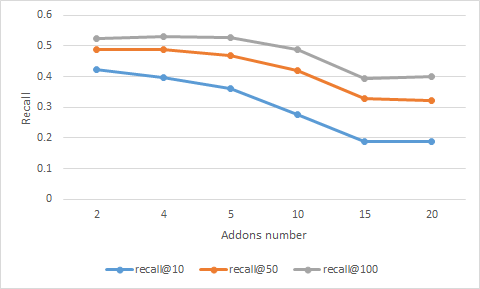
\includegraphics[scale=1,angle=0]{figures/addonsNumberGraph.png}
\caption{Effect of query size on prediction accuracy}
\label{fig:addonsNumberGraph}
\end{figure}


\iffalse We have also verified that user nodes are crucial for the prediction
algorithm, as shown in \autoref{fig:nouserNoremove}.

\begin{figure}[!htbp]
\centering
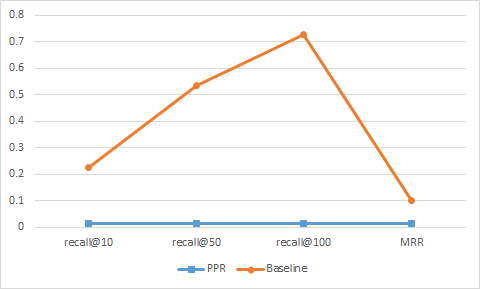
\includegraphics[scale=.8,angle=0]{figures/nouserNoremove.png}
\caption{Effect of user nodes on prediction accuracy}
\label{fig:nouserNoremove}
\end{figure}
\fi

\section{Discussion}

In this chapter, we evaluated the coherence among addons that are installed on the same machine. We found that Personalized PageRank performs well on the task of predicting relevant addons given information about its environment. Alternative one-fit-all rankings of addons by popularity or graph centrality yielded substantially inferior results, indicating that addon populations exhibit strong correlations between individual addon species.  

We haven't yet examined the reasons for the existence of these correlations. Multiple factors may underlie this phenomenon. The mixture of addons on one's machine is certainly affected by the user's personal preferences, as long as the user is actively involved in maintaining his computing environment. Another factor is functionality, where some addons are complimentary. Importantly, and of high interest, are positive correlations between addons as the result of interventions and manipulations of software companies in the add installation process. Co-existence of addons by different companies may be an indication of  business alliances. Moreover, rivalry between addon distributors may be reflected in negative correlation between these addons. In the next chapter, we investigate business alliances and rivalries as factors that explain trends observed in the addon ecosystem.  

\chapter{PPR-based analysis of addon coexistence}
\label{chap:Symbiosis}

In this chapter, we investigate the addon coexistence phenomenon. We observe that existence of some addons on a user's machine tends to be affected by other addons, i.e. when addons of one company are installed, addons of another company have greater or lower chances to be installed on the same machine. The positive effect of coexistence will hereafter be called \emph{symbiosis}, while the negative effect will be called \emph{clash}.

The symbiosis phenomenon often occurs when addons of some companies are distributed via third parties: addon installation is offered to a user as a part of some other product installation process, for example, while the user installs Skype, the installation process suggests also installing Skype's `Click to Call' addon in all browsers. Another example is Ask Toolbar: at the time the data for this chapter was collected, Ask Toolbar installation was integrated with Java installation\footnote{\url{https://java.com/en/download/faq/ask_toolbar.xml}}. During the installation of Java, users were prompted to download and install the Ask Toolbar, see \autoref{fig:ask_offer}. 

The clash effect can be observed when addons of one company get removed if addons of another company are installed on this machine or if the addons are not installed at all when another's company addons are pre-installed on the machine. For example, \emph{Kaspersky AntiVirus}, which develops addons for all browsers, treats \emph{iMesh} addons as threats and removes them from the computer\footnote{\url{http://securelist.social-kaspersky.com/en/kadvisories/KLA10420}}.

Needless to say, the life cycle of the addon ecosystem is mostly obscure for an outside observer. While some symbiotic effects are fairly visible to the users (e.g., an addon is prompted to be installed during an installation processes of another addon or a software product), some other symbiotic effects are hidden (e.g., those following undisclosed agreements between addon distributors). Clash effects, on the other hand, are almost always invisible. Besides a few well known conflicts between competing addon distributors that were widely covered in mass media\footnote{\url{http://goo.gl/AdlzUM}}, the competition is kept away from the eyes of general public. In this chapter, we disclose some of these effects and shed light on the entire addon ecosystem. 

\begin{figure}[!htbp]
\centering
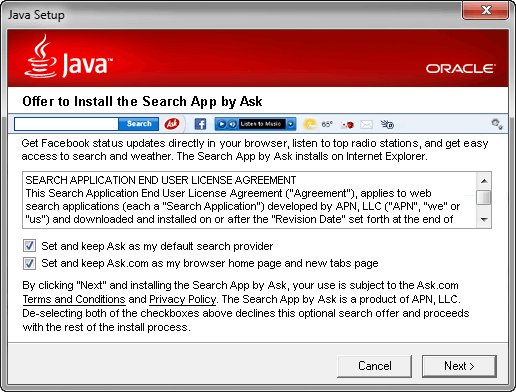
\includegraphics[scale=.8,angle=0]{figures/ask_offer.png}
\caption{ASK Toolbar installation bundled with Java version upgrade.}
\label{fig:ask_offer}
\end{figure} 

The ability to detect a symbiosis or clash between addon distributing companies could turn handy for addon owners. Information about symbiosis between two companies can help a third company to better analyze the powers and driving forces of the addon market, and to get better prepared for a potential competition. While it is unlikely that a company would not be aware of symbiosis between its own addons and addons of another company, information about a clash that involves the company's addons can sometimes come unexpected. A typical addon manufacturer can benefit from information about a clash between their own and someone else's addons in four ways:
\begin{enumerate}
\item Such a clash may imply that the user prefers someone else's addon over their own addon, so there might be a way to perform a comparative analysis of the two addons and learn how to improve their value proposition.
\item The clash could mean that a newly installed addon is hostile to other addons in an illegal way, i.e. it is the addon --- and not the user ---- that uninstalls or sabotages another addon. Then, the distributor of the removed addon could report an abuse to the webstore owner.
\item An addon developing company can ask a third-party distributing company not to install their addon on a machine that keeps the hostile addon. Since in most cases addon developers are paying distributors per install, this could decrease the developers' costs and improve their profits in a long run.
\item A clash can occur between addons of seemingly non-competing companies. This can happen when something goes wrong in the distribution process and the problem slips off the company's radar. The addon ecosystem is complex enough to make the distribution monitoring barely possible. If an unintended clash gets detected, the owner of the affected addon can contact the owner of the hostile addon and ask them to act.
\end{enumerate}

%\section{Experimental setup}
We chose nineteen companies (see~\autoref{table:companies_list}) among well-known addon distributors. These are companies that are most ``famous'' among the distributors of addons and toolbars. Interestingly, seven of the nineteen companies are antivirus and anti-malware companies. 
Although antivirus and anti-malware software aim to prevent unintentional addon installation, some antivirus companies are not only fighting unintentional addon installations but also distributing their own addons and toolbars. For example, AVG Anti Virus company distributes the AVG Security Toolbar which is detected by Avast Anti Virus as malware.  

In 2013, Avast Anti Virus published a list of top ten companies that were distributing their addons via third-party software installations\footnote{\url{https://blog.avast.com/2013/03/20/avast-browser-cleanup-at-work/}} --- these addons were subject to removal. Surprisingly, the list published by Avast in 2015 is very similar to their 2013 list --- many of these companies are in our list as well~(\autoref{table:companies_list}). Back in 2013, Avast identified over 3,300,000 different browser extensions for three major browsers. They also noticed that ``A lot of toolbars are available in different variants. These variations affect mostly the name''. 

In a blog post of July the 9th 2015, Avast describes the addon ecosystem of a user's Web browser. They mention that one of the major characteristics of the ecosystem is that ``the addons fight against each other''\footnote{\url{https://blog.avast.com/2015/07/09/top-10-most-annoying-browser-toolbars/}}.
Based on Avast statistics on forced removals of competing toolbars, some companies from our list are among the top ten offenders. For example, Conduit performed more than 13,000,000 removals of their competitors' toolbars, ASK removed 11,000,000 toolbars and other companies were not far behind. Not surprisingly, Avast itself uses the same practice. A Techdows blog post\footnote{\url{http://techdows.com/2012/11/avast-comes-bundled-with-google-toolbar.html}} mentions that ``Avast is contradicting itself. Their latest product offers a built-in feature to rid your browser of toolbars, while offering a toolbar when installing their software.''

To the best of our knowledge, this thesis is the first research study of the addon ecosystem in the Web browser. This is a true Big Data study as we analysed Web browsers of close to a million users. Both addon developers and computer security companies can benefit from this study and its conclusions. In the rest of this chapter, we will describe the setup of our empirical analysis, in particular, the reasons behind our design choices. We will provide background information and cover the history of this project starting with preliminary experimental efforts we made before coming up with our final experimental design. We will then present our main findings: the identified symbiosis and competition relationships. We will conclude this chapter with a discussion on the results.

% Please add the following required packages to your document preamble:
% \usepackage{booktabs}
\begin{table}[!htbp]
\centering
\caption{Companies list}
\label{table:companies_list}
\begin{tabular}{@{}lll@{}}
\toprule
{\bf Company name} & {\bf Example Product}               & {\bf Description}               \\ \midrule
ASK                & Ask Toolbar                 & Advertisement/Search company    \\
AVG                & AVG Safe Search add-on      & AntiVirus/Advertisement company \\
Avira              & Avira Browser Safety        & AntiVirus company               \\
Babylon            & Babylon Toolbar             & Advertisement/Search company    \\
Blekko             & Blekko Toolbar              & Advertisement/Search company    \\
Conduit            & Conduit Toolbar             & Toolbar provider company        \\
Google             & Google Toolbar              & Advertisement/Search company    \\
Hotspot Shield     & Hotspot Shield VPN          & Security company                \\
iMesh              & iMesh Search                & Advertisement/Search company    \\
Incredimail        & MyStart by Incredimail      & Advertisement company           \\
Kaspersky          & Kaspersky Protection Plugin & AntiVirus company               \\
Montiera           & Montiera Toolbar            & Toolbar provider company        \\
Norton             & Norton Toolbar              & AntiVirus company               \\
Softonic           & Softonic Web Search         & Advertisement company           \\
SpeedBit           & Video Accelerator           & Software company                \\
SweetIM            & SweetIM Toolbar             & Advertisement/Search company    \\
Trend Micro        & Trend Micro Toolbar         & AntiVirus company               \\
Zone Alarm         & Zone Alarm Toolbar          & AntiVirus company               \\ 
Zugo               & Search Toolbar              & Advertisement company           \\ \bottomrule
\end{tabular}
\end{table}

\iffalse
At first, we have tried to classify add-ons clash with Support Vector machine, but we saw no signal and the SVM could not converge. [Need much more info here - RON, UPDATE: did we actually use SVM for predicting clash? I think we used SVM to predict an addon survival which is mainly affected by the user behavior. Anyhow, I would love to see a paragraph explaning what we did back then.]
\fi

\subsection{Preliminary Experimentation Efforts: Addon Survival Prediction}
Initially, our experimentation efforts were concentrated on addon \emph{survival prediction}. On an example of one addon development company, Speedbit, we aimed to identify Web browsers whose ecosystem allowed Speedbit addons to survive for an extended period of time, in contrast to those browsers where Speedbit addons tended to get uninstalled quickly. We approached the survival prediction task within the Machine Learning framework of \emph{binary classification}~\citep{sebastiani02}. In binary classification, a prediction model is trained on labeled data of two classes: positive instances and negative instances. We constructed our training data as follows: browsers in which Speedbit addons survived for three or more days were considered positive instances---all other browsers were considered negative instances. 

Each browser was represented as a feature vector that was constructed based on the set of addons installed on that browser. Each addon's name, full path, and textual description (see~Section~\ref{sec:methods}) were split to single words, and a simple Bag-Of-Words model of an addon was constructed. A browser's feature vector was then aggregated from Bags-Of-Words of all addons installed on that browser. We used the popular libSVM tool~\citep{chang2011libsvm} to learn a Support Vector Machine classifier on the training set of browsers' feature vectors.

We split our dataset to $2/3$ training set and $1/3$ test set (uniformly at random). Since we had about 900,000 browsers in our dataset, our training set consisted of about 600,000 browsers. This training set turned out to be too large for the non-parallelized libSVM. After a few unsuccessful attempts to train the model on the entire training set, we decreased its size by taking all positive instances and a random sample of $1/3$ of negative instances.

The results were not encouraging. Only in about 20\% of browsers in which Speedbit addons were predicted as surviving, the addons actually survived. Moreover, only about 5\% of browsers where Speedbit addons survived were identified by our system. A possible explanation for such a poor performance of our system is the fact that modeling addon survival as a binary classification task might be too coarse: some addons survive for longer time and some survive for shorter periods, so the regression modeling framework might be a better option for the task in hand. Another explanation might be in a specific parameter setting that we did not manage to achieve. After some consideration, we abandoned the addon survival prediction task altogether.

\iffalse
Running training libsvm on the new samples took one hour.
optimization finished, iter = 41654
nu = 0.706971
obj = -196797.924484, rho = 1.994601
nSV = 40041, nBSV = 39227
Total nSV = 40041
Then we've decided to find another way to represent our data.
\fi

\section{Experimental design}
\label{sec:experiment_des}

In this work, we research coexistence effects in the addon ecosystem. In~\autoref{chap:user_ecosystem}, we investigated the addon ecosystem on the individual level: if a subject (an addon) is artificially extracted from a web browser of a specific user, the browser ecosystem ``knows'' which subject is missing. In this chapter, in contrast, we analyze coexistence of \emph{addon manufacturing companies}, i.e.~\emph{species}, using the ecological parlance. 

In the new setting, we first need to reveal which addon belongs to which company. An addon company most often distributes many addons --- hundreds or even thousands. For example, \emph{Kaspersky URL Advisor Firefox addon} and \emph{Kaspersky Protection Chrome extension} are developed by the same company, so we say that they belong to the same species. Often, the same addon has different names --- it is not easy to infer that addons with different names are in fact the same addon. We do not aim to infer that --- instead, we are concerned with mapping addon names to company names. Also, it is important to mention that addons bear characteristics of a machine on which they are installed. For example, the file-system path of an addon on a specific machine may or may not be unique among all addons we observe in this study: a user can choose to install an addon at a non-standard location in his/her machine's file system, or stick to a default location instead.

As discussed in Section~\ref{sec:methods}, an addon is represented in our system by three data attributes: the addon's name, the full file-system path of its installation, and a textual description. Any one (or any two but not all three) of the attributes may be empty. To infer which addon belongs to which company, we first apply a simple heuristic of detecting the company name within the three attributes of an addon. The rationale behind this is that the default path of an addon package installation often contains the company's name. If a user does not decide to change the default option, the company name will most probably be detected in the addon's path. In addition, the name and the description fields may contain the company name as well, see \autoref{table:addon_desc} for an example.

% Please add the following required packages to your document preamble:
% \usepackage{booktabs}
\begin{table}[!htbp]
\centering
\caption{An example of a company's name contained in an addon's path or description}
\label{table:addon_desc}
\begin{tabular}{@{}|l|l|@{}}
\toprule
Path & C:\textbackslash{Program Files (x86)}\textbackslash{Kaspersky Lab}\textbackslash{Kaspersky Internet Security 2012}\textbackslash{avp.dll} \\ \midrule
Description & Kaspersky Protection extension \\ \bottomrule
\end{tabular}
\end{table}

After applying the company name search heuristic, we realized that representations of many addons that belong to companies from our list~\autoref{table:companies_list} do not in fact contain the company name. For example, an addon $tbbaby.dll$ doesn't contain company name in any of its attributes, but does belong to Babylon\footnote{\url{http://www.shouldiremoveit.com/Babylon-English-Toolbar-31094-program.aspx}}. 
We propose the following procedure, see algorithm \autoref{alg:find_addon_species}, for mapping this kind of addons to their owners. 

In ~\autoref{chap:user_ecosystem}, we applied a Personalized PageRank (PPR) based algorithm for identifying a missing addon in a browser of a specific user. We proposed a method that took the entire set of the user's addons as a query input to PPR and produced the output of a ranked list of all addons in the system. We hypothesized that the missing addon would end up among the top addons in the ranked list. Our hypothesis was proved correct.

We apply a similar method here, for mapping addons to their manufacturer companies. 
As in ~\autoref{chap:user_ecosystem}, we are applying the PPR based algorithm on a graph with user, addon, and term nodes. An individual user's node is linked to the set of nodes each one corresponding to an addon installed on the user's machine. The addon nodes are linked to their corresponding user and term nodes. As described in~\autoref{sec:design}, we experimented with a few versions of the graph, where our design choices were the existence or absence of high-degree nodes, the usage of term nodes and of addon full path information. In this chapter, we experiment with the graph as described in \autoref{sec:user_main_results}, i.e.~the graph with all addons (without removing the high-degree addons or term nodes), however we do remove the addon file-system paths\footnote{Addon paths are instrumental for mapping addons to companies using the simple heuristic described above, however, for the PPR purposes, addon paths turn out to be too noisy to deal with, and are thus removed.}. We never change the graph setting over the course of this chapter.

As a query for the PPR algorithm, instead of the set of addons existing in a user's browser, we now provide a set of addons that are known to belong to a company. We hypothesise that an addon that belongs to that company, and is not in the query, would ``pop-up'' in the ranked list. By ``popping-up'' we mean that the addon would be ranked closer to the top of the list, relatively to its original rank in the (non-personalized) PageRank. First, we run the non-personalized PageRank on the entire graph, and use the rank of each addon as the baseline position. For each company, we then run the Personalized PageRank and identify addons that drastically change their position in the ranked list. For example, if an addon was at a rank of 15 in the non-personalized PageRank and moved to the rank of 14 in the PPR, we do not take it into account as its rank did not dramatically change. In contrast, if an addon was at a rank of 100 in the non-personalized PageRank and moved to the rank of 10 in the PPR, we consider it as a candidate to manual examination. For each addon that ``popped-up'' in the ranked list of a specific company's PPR, we manually validate that the addon actually belongs to the company.

We perform the procedure described above iteratively: after we discover addons that belong to a company, we add them to the query and rerun the PPR with the extended query. We stop the process once there are no more addons that dramatically change its rank. It turns out that two iterations are enough for the process to converge. Using this process, we discover 24 addons that ``popped up'' in the PPR ranked lists of companies from~\autoref{table:companies_list}. In a manual check of these 24 addons, we see 100\% precision: there was not one single addon we checked that did not after all belong to the company in the query. 

\begin{algorithm}[!t]
\caption{Finding addon relation to Company}
\label{alg:find_addon_species}
\begin{algorithmic}[1] 
\REQUIRE Graph $G$, teleportation vector $v$, company name $n$
\STATE Run Personalized PageRank on graph $G$, with seed node from $v$.
\STATE Rank the addons according to $PPR_gscore$, i.e. the Personalized PageRank scores after run
\FOR{each addon node}
\STATE Compare $PPR_gscore$ with $PR_gscore$
\IF{$PPR_gscore$ $\gg$ $PR_gscore$}
\STATE This addon could be related to the company - check manually
\ENDIF
\ENDFOR
\end{algorithmic}
\end{algorithm}

An example for an addon that drastically changed its rank is the addon named \emph{tbmyba.dll}, which jumped from the 1200 rank position to the 15 rank position when running PPR with Babylon addons in the query. Indeed, we found out that this addon belongs to Babylon\footnote{\url{http://www.file.net/process/tbmyba.dll.html}}.

The success of this process reveals an interesting phenomenon: it turns out that there is a ``community'' of addons of the same company, and this community can be discovered via the Personalized PageRank weight propagation that starts with already known community members. One possible explanation for this phenomenon would be that it is a common practice for a company to offer a few of its addons for installation at the same time. For example, while Babylon is installing its Internet Explorer addon, it might also install its Chrome extension. Even if we manage to map the Internet Explorer addon to Babylon using the simple name matching procedure, the Chrome extension might not contain any attribute that would qualify it as related to Babylon. Still, our algorithm would discover it in a similar way it discovered a missing addon for a specific user. 
Another explanation may come from the \emph{collaborative filtering} theory, described in \autoref{sec:recommender_systems} and \autoref{sec:user_profilingg}: users who have many addons in common might also have different addons of the same company --- such addons will therefore be located in a close proximity of each other in the PageRank graph.

Now that we linked addons with their species (that is, their manufacturer companies), we are ready to analyze relations between the addon companies in the Internet ecosystem. The following algorithm~\autoref{alg:collect_addon_data} summarizes our methodology. 
For each company from our list, we construct the PPR query to contain all the company's addons. The PPR output is the ranked list of all addons in the graph. Our goal is to find out addons of which companies ``pop up'' in the PPR as compared to non-personalized PageRank. If we identify a company whose addons are universally improving their rank in the PPR of another company, we may conclude that the two companies are engaged in a partnership. Using the ecological language, we call it \emph{symbiosis}. We also expect addons of some companies to ``drop down'' the PPR ranked list, in comparison to the regular PR ranked list. We can suggest that two companies \emph{clash} with each other if many addons of one company drop down in the PPR of another company.

\begin{algorithm}[!t]
\caption{Addon company coexistence}
\label{alg:collect_addon_data}
\begin{algorithmic}[1] 
\REQUIRE Graph $G$, Companies $COMP$
\STATE Run PageRank on graph $G$
\FOR{company $c\in COMP\ $}
\STATE Define personalization vector $v$, with seed nodes as all addons $\in COMP\ $
\STATE Execute Personalized PageRank
\STATE Rank all addons according to the PPR score
\FOR{company $d\in COMP \setminus \{c\} $}
\STATE Compute expected PPR score 
\STATE Compare with expected PR score
\STATE If there is a significant drop $\Rightarrow$ clash
\STATE If there is a significant increase $\Rightarrow$ symbiosis
\ENDFOR
\ENDFOR
\end{algorithmic}
\end{algorithm}

\section{Analysis}
\subsection{Symbiotic Relationships}
\label{sec:symb_relations}

\subsubsection{Addon Co-occurrence}
\label{subsub:co_occurrence}

Generally speaking, there may be multiple ways to detect symbiosis between addon manufacturing companies. One could suggest a simple way for detecting a symbiotic relationship which would be based on computing co-occurrence frequencies of addons on users' machines. If many addons of company $c_i$ are installed on the same machines where addons of company $c_j$ are installed, we may conclude that the two companies live in symbiosis with each other. To validate this hypothesis, we set up a simple experiment. For each pair of companies from our list (\autoref{table:companies_list}), we computed Jaccard index~\citep{jaccard1912distribution} which is the measure of overlap of two sets. We denote $\mathbf{M}_i$ the set of machines on which addons of company $c_i$ are installed. Analogously, we denote $\mathbf{M}_j$ the set of machines on which addons of company $c_j$ are installed. Jaccard index is then defined as:
$$
Jaccard(c_i, c_j) = \frac{|\mathbf{M}_i \cap \mathbf{M}_j|}{|\mathbf{M}_i| + |\mathbf{M}_j| - |\mathbf{M}_i \cap \mathbf{M}_j|},
$$
where the absolute value symbol means the cardinality of a set.

\begin{figure}[!htbp]
\centering
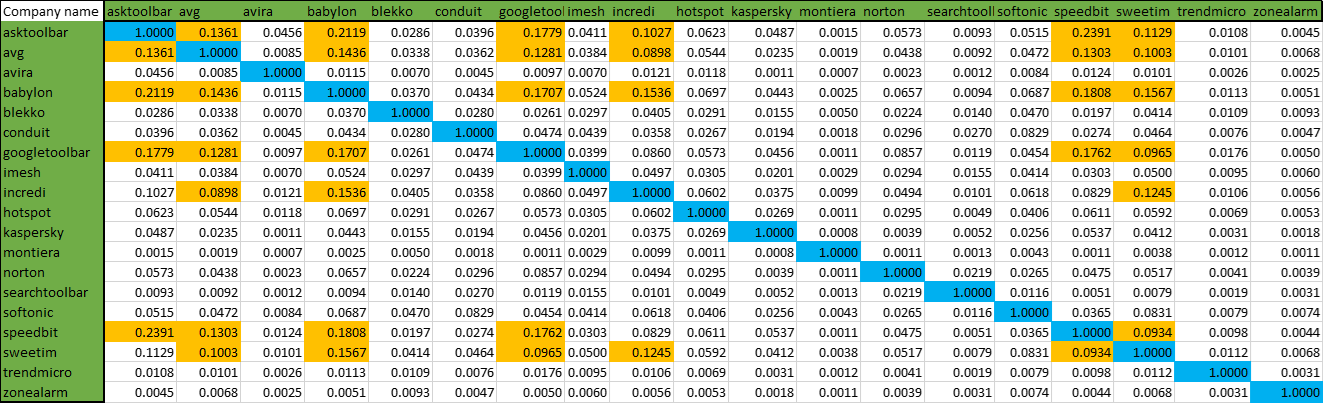
\includegraphics[width=\linewidth]{figures/JaccardMatrix.png}
\caption{All companies Jaccard index}
\label{fig:jaccard_matrix}
\end{figure}

The full matrix of Jaccard indexes is presented in~\autoref{fig:jaccard_matrix}. As we can see, some pairs of addon manufacturing companies have quite a significant co-occurrence, comprising of up to 24\% machines on which the two companies' addons are installed (taken as a union). 

Somewhat counter-intuitively, the most significant co-occurrences do not appear corresponding to known collaborations between addon distributors. Even more counter-intuitively, some significant co-occurrences correspond to known competitions between addon distributors. An example is ASK, AVG, Google, and Babylon, all of which heavily co-occurring in our dataset. The four companies are distributing their own toolbars, thus competing with each other \footnote{\url{http://www.thewindowsclub.com/uninstall-babylon-yahoo-google-bing-toolbar}}. Moreover, some companies such as IncrediMail and Conduit, which are known for cooperation between them\footnote{Conduit eventually acquired IncrediMail, see~\url{http://goo.gl/4dybI6}.}, do not co-occur heavily.\footnote{These observations are correct for 2013 when our data was collected. Since then, the addon ecosystem has undergone many changes, e.g. Babylon shut down and Google stopped distributing its own toolbar. Still, most of the other players in the domain exist and there are some other new companies as well, see \url{https://blog.avast.com/2015/07/09/top-10-most-annoying-browser-toolbars/}}.

A possible explanation for heavy co-occurrence of competing toolbars is actually in the intensity of the competition: major toolbar manufacturers are all working hard on ``sneaking in'' as many machines as possible. They all have very strong distribution mechanisms that allow a constant increase in their market penetration. While their toolbars get installed on many machines, they do not necessarily ``kick out'' toolbars of their competitors. Moreover, a direct clash is pretty rare because of enormous resources it would require given the size and significance of competing companies, and potential legal implications. Therefore, multiple toolbars get installed on the same machine, which is mostly the function of the user's tolerance: some users do not care / are not aware of / do not know how to prevent multiple toolbar installations. This leads to high co-occurrence of toolbars on some machines, but does not in the end indicate any collaboration between the toolbar distributors.

To summarize, addon co-occurrence computation does not appear to be the correct way to reveal symbiotic relationships between addon distributors.

\subsubsection{Personalized PageRank}

Following~\autoref{chap:user_ecosystem} and~\autoref{sec:experiment_des}, we use Personalized PageRank as the main mechanism to detect company symbiosis in the Web browser ecosystem. Addon ranking obtained by the standard (non-personalized) PageRank corresponds to the unbiased and undisturbed addon ecosystem in which every addon bears its relative importance value with respect to the others. Once the personalized PageRank is applied, the ecosystem is disturbed with artificial preference of some of its elements. The artificial disturbance causes the entire ecosystem to adjust to the new condition, and such an adjustment reveals characteristics of the ecosystem that would not be visible in the original, undisturbed state. 

\iffalse
\begin{figure}[!htbp]
\centering
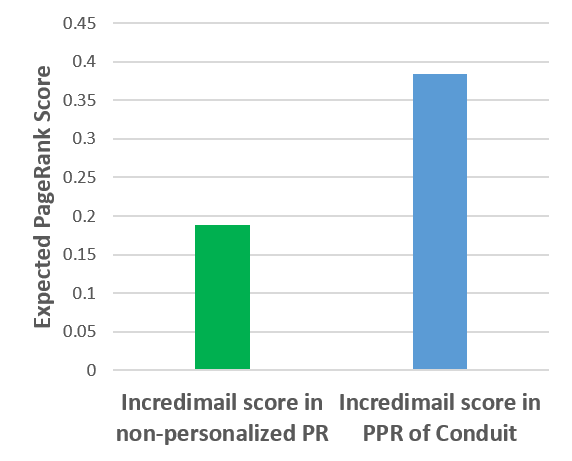
\includegraphics[width=\linewidth]{figures/incredi_sym_conduit.png}
\caption{IncrediMail symbiotic relation with Conduit}
\label{fig:incredimail_sym_conduit}
\end{figure}

\begin{figure}[!htbp]
\centering
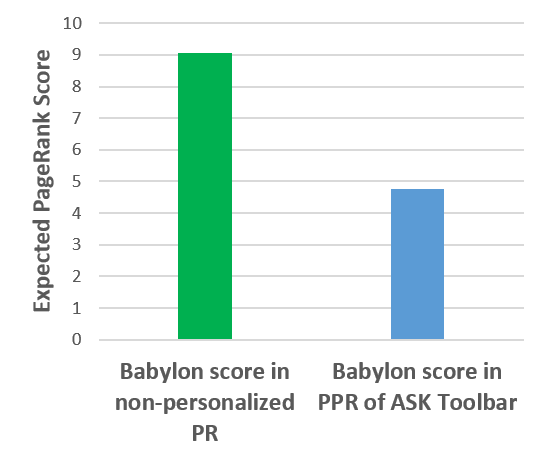
\includegraphics[width=\linewidth]{figures/babylon_nosym_ask.png}
\caption{Babylon non-symbiotic relation with ASK Toolbar}
\label{fig:babylon_nosym_ask}
\end{figure}
\fi

When all addons of a particular company comprise the PPR query, it is natural to expect the company's addons popping up in the ranked list. Other addons that are closely related to the addons of the query company might then follow the company's addons in their way to the top of the ranked list. The beauty of personalized PageRank is in the fact that the essence of the relationship between the addons does not have to be disclosed a priori, nor explicitly modeled. This implies that hidden, invisible relationships between addon manufacturers can be discovered in the process.

Our research hypothesis is that addons that pop up in the PPR ranked list belong to a company $C_i$ that is involved in a symbiotic relationship with the query company $C_q$. Our goal is to reveal such a relationship based on the $C_i$'s addon behavior as a reaction to the PPR disturbance of the addon ecosystem. Since companies usually maintain many addons, we cannot expect any company to have all its addons universally popping up in the ranked list once PPR is applied. Obviously, some addons would pop up higher than the others, while some addons might not change their rank substantially, or even drop down the ranked list. If we measure the rank change of addons that belong to $C_i$, we could make a conclusion about the probability of a symbiotic relationship between $C_i$ and $C_q$.

There are two factors that affect the significance of the addon's rank change:
\begin{enumerate}
\item \textbf{Length of the leap.} Obviously enough, the longer is the addon's leap from the original rank (in non-personalized PR) to the new rank (in PPR), the more significant the rank change is.
\item \textbf{The (final) PPR rank.} The length of the leap is not the only significance measure. Intuitively, if an addon jumps from rank 10,000 to rank 1000, such a jump is less significant than if the addon jumps from rank 100 to rank 10. The explanation is simple: an addon at a rank 10,000 was most probably not important, and a big change in its rank would not make it significantly more important. In contrast, an addon that moved to the 10th place cannot be ignored.
\end{enumerate}

We are interested in the change of rank of the company, as aggregated over the set of its addons' ranks. In a search for a formula that would aggregate the behavior of all the company's addons, we make the following observation: if an addon is rare (i.e.~installed on just a few browsers), then the change in its rank --- even a significant one --- might have little effect on the behavior of the company in whole. For example, if an addon moves from rank 10,000 to rank 10, but is installed on 10 user browsers only, its effect on the aggregated rank of the company would be less significant than, say, a change in rank from 100 to 50 of an addon that is installed on 10,000 user browsers.

The potential complexity of addon rank aggregation over the three parameters listed above (length of the leap, the final rank, and the addon frequency) makes us search for simplification. Since an addon's rank is determined by the order of all addons when sorted over their PR (or PPR) \emph{scores}, we observe that an addon score is a better measure of the addon's importance than its rank. For example, if an addon's score was 5 in the non-personalized PR, and got increased to 10 in PPR, while there were no other addons with scores as high as 5, then the rank of the addon would not change, so the significance of the score change would be completely ignored when taking into account addon ranks only. In addition, the change in the addon's rank is affected by the change of other addons' ranks, while the change of the addon's score can be taken independently from the other addons' score change. Therefore, we decide to focus on addon PR scores rather then on ranks. Now, there are only two parameters that need to be taken into account for measuring a company's ``importance'': the PR (or PPR) scores of its addons, and their frequencies in the dataset.

We estimate the ``importance'' of company $c$ by its \emph{expected} PR score, which is the weighted sum of PR scores of the company's addons. Let us denote $s_i$ the PR score of addon $a_i$ that belongs to the set $\mathbf{A}_c$ of all addons of $c$. The expected score $S_c$ (of the company $c$) will then be:
$$
S_c = \sum_{a_i \in \mathbf{A}_c} p_i s_i
$$
where $p_i$ is the probability of drawing addon $a_i$ from all $c$'s addons. Specifically, we define $p_i = freq(a_i) / freq(\mathbf{A}_c)$, where $freq(a_i)$ is the frequency of addon $a_i$ in terms of the number of user browsers on which $a_i$ is installed; $freq(\mathbf{A}_c)$ is the sum of frequencies of all $c$'s addons.

%After running the PPR with all addons of a company $C_q$ in the query, we first remove $C_q$'s addons from the ranked list in order to make a clean experiment: depending on the number of addons $C_q$ is maintaining --- and their original PR ranks --- their PPR ranks can significantly affect the change in ranks of other addons. We want to eliminate this influence and focus on the rank change of the other companies' addons. That is why we remove $C_q$'s addons both from the PPR ranked list and from the original PR ranked list.

%We examine the top 100 addons (after removing $C_q$'s addons), and compare their ranks to their original PR rank. For each company other than $C_q$, we [RON:Here] only addons that have more than 100 users, only nodes that belong to the companies of interest, 

%Add the formula that describes relative jump. Expected score

\begin{table}[t]
\centering
\caption{Expected PageRank scores}
\label{table:pagerank_scores}
%\resizebox{\textwidth}{!}{%
\begin{tabular}{@{}lllll@{}}
\toprule
 & \textbf{\#addons} &  \textbf{Expected PageRank score} &  \\ \midrule
\textbf{ASK} & 229038 & 3.930655827 \\
\textbf{AVG} & 131337 & 1.458013998 \\
\textbf{Avira} & 10624 & 0.165028673 \\
\textbf{Babylon} & 191386 & 9.064855902 \\
\textbf{Blekko} & 14381 & 0.147602568 \\
\textbf{Conduit} & 21671 & 0.188175047 \\
\textbf{Google} & 187455 & 3.327125475 \\
\textbf{iMesh} & 23954 & 1.439130402 \\
\textbf{IncrediMail} & 76198 & 2.375531006 \\
\textbf{Hotspot} & 54675 & 1.053817694 \\
\textbf{Kaspersky} & 47793 & 0.849401341 \\
\textbf{Montiera} & 809 & 0.017516 \\
\textbf{Norton} & 53826 & 1.078813495 \\
\textbf{Searchtoolbar} & 5169 & 0.043609128 \\
\textbf{Softonic} & 29410 & 0.274080246 \\
\textbf{SspeedBit} & 484676 & 7.540780048 \\
\textbf{SweetIM} & 84871 & 1.445297894 \\
\textbf{TrendMicro} & 10325 & 0.155437633 \\
\textbf{ZoneAlarm} & 3597 & 0.030242981 \\ \hline
\end{tabular}
%}
\end{table}

\iffalse
A personalized PageRank vector is the stationary distribution of a random walk that, with probability $\alpha$ follows a step of a random walk and with probability $(1-\alpha)$ jumps back to a seed node. When there are multiple seed nodes, then the choice of the seed node is uniformly random. Thus, nodes close to the seed are more likely to be visited and get a higher rank. Recently, such techniques were shown to produce communities that best match communities found in real-world networks~\citep{abrahao2012separability}. Putting company nodes as the only seed nodes in personalized PageRank will grant a higher score to the company addons and the addons that are related in some way to this company. Our hypothesis is that nodes of the company that are having symbiotic relation with the seed nodes company will also get a higher score because of its relatedness to the symbiosis company.
\fi

We aggregate PageRank scores of all addons of a company into the expected PageRank score (see~\autoref{table:pagerank_scores}). For each company $c_q$ in the PPR query, we compute the expected PPR scores of all the other companies. 

%In addition, we maintain a ranked list of companies according to their expected (non-personalized) PR scores (see~\autoref{table:pagerank_scores}). For each $c_q$, we compare the two ranked lists of companies. If a company $c_i$ ``pops up'' closer to the top of the $c_q$'s PPR ranked list of companies, as compared to the original (non-personalized) ranked list of companies, we conclude that $c_i$ and $c_q$ are in a symbiotic relationship. 

%[SELA: Added Ratio Matrix, \autoref{fig:RatioMatrix}. The red cell are the ones with ratio smaller than 1, the red cells with border are the ones smaller than 0.5. The green cells are the ones with ration greater than 1, the green cells with border are the ones greater than 1.1]
\autoref{fig:RatioMatrix} shows the ratio between expected PPR scores of company $c_i$ given a query company $c_q$ and the expected non-personalized PR score of $c_i$. Ratios greater than 1 are colored in green, all the rest is colored in red. It can be immediately seen that most ratios are colored in red, meaning that PPR scores are generally lower than PR scores. Some cells of the table are highlighted with a dark frame. Green cells are highlighted if the PPR to PR ratio is greater than $1.1$, while red cells are highlighted if the PPR to PR ratio is lower than $0.5$. Those cells correspond to company pairs that are likely to stay in a symbiotic (green) or clash (red) relationship with each other.

It is inevitable to notice that the score ratios in~\autoref{fig:RatioMatrix} are not symmetric, i.e.~the expected PPR score of company $c_1$ can decrease when $c_2$ is in the query, however, the expected PPR score of $c_2$ can increase when $c_1$ is in the query. This can be easily explained by non-symmetry of symbiotic / clash relationships: two companies $c_1$ and $c_2$ can sign a contract according to which $c_1$ helps distributing addons of $c_2$, however $c_2$ does not have to help distributing addons of $c_1$. Moreover, $c_2$ may even end up removing $c_1$'s addons. 

\begin{figure}[!htbp]
\centering
    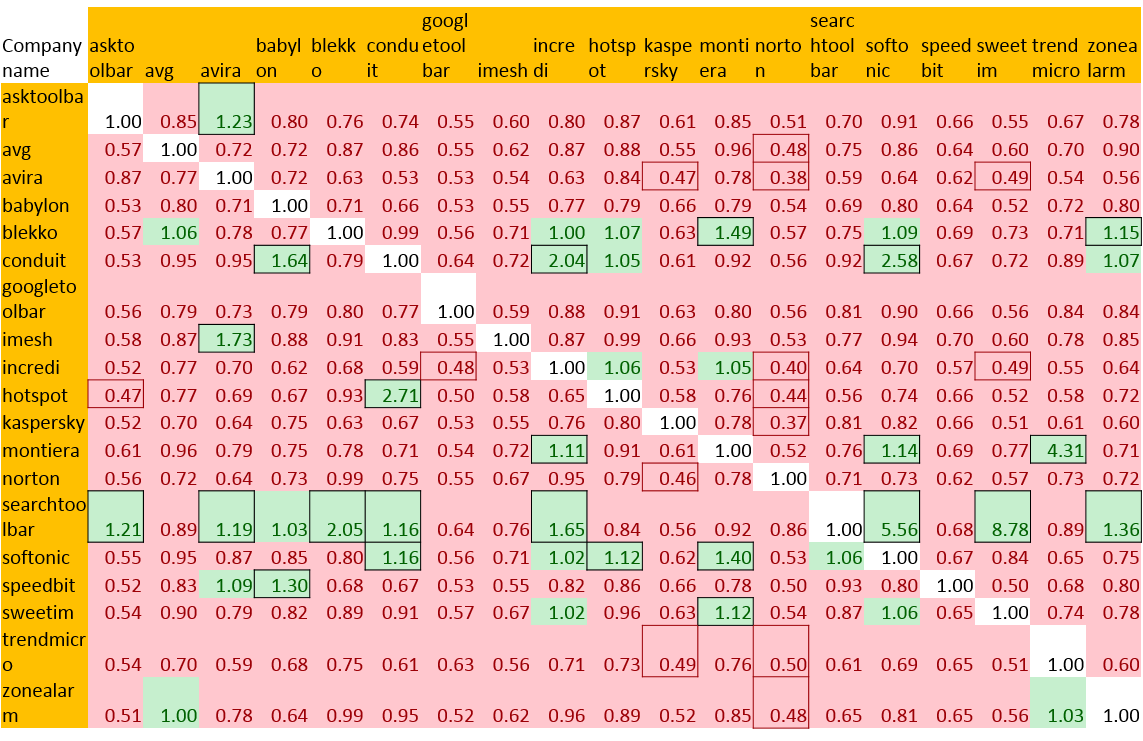
\includegraphics[scale=0.8]{figures/RatioMatrixPortrate.png}
    \caption{Ratios of Expected PPR and expected PR scores of companies. Rows are companies in PPR queries.}
    \label{fig:RatioMatrix}
\end{figure}

%By a quick look at the \autoref{fig:RatioMatrix} relations, we see that some companies are more "friendly" with others, e.g. given SearchToolbar company the expected PPR scores from Softonic and SweetIM are greatly improved. This could be explained by many distribution agreements the SearchToolbar company (Zugo) has signer  There also company that one hurts others performance, e.g. given the Norton anti virus company, all others companies expected PPRs scores are hurt. This behavior can be explained by the essence of any anti virus company - not favoring addons distributors. Some exceptions are anti virus companies like Avira which has bundled with addons manufacture like ASK.

Our methodology appears very successful in revealing truly symbiotic relations between companies. Below are a few examples. Their PPR to PR ratios are can be seen in~\autoref{fig:RatioMatrix}, however we prefer to also show a separate figure per example.

In~\autoref{fig:incredi_sym_conduit}, we show the expected score of IncrediMail in Conduit's PPR and its expected score in non-personalized PageRank. We can see that IncrediMail's score increases significantly when PageRank is personalized around Conduit: as the personalized PageRank prioritizes Conduit, it also ``drags up'' IncrediMail. This implies that there is a close semantic relationship between Conduit and IncrediMail: as we mentioned in~\autoref{subsub:co_occurrence}, Conduit ended up merging with IncrediMail (which is now called Perion) in 2014. 

\begin{figure}[!htbp]
\centering
\begin{subfigure}[b]{0.8\textwidth}
	\centering
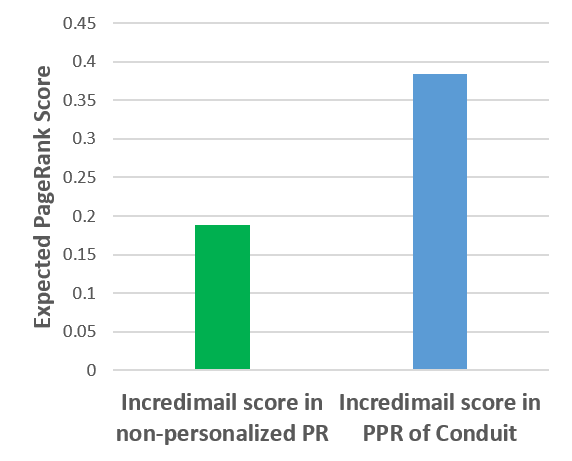
\includegraphics[scale=0.8]{figures/incredi_sym_conduit.png}
\caption{IncrediMail symbiotic relation with Conduit}
\label{fig:incredi_sym_conduit}
\end{subfigure}
\begin{subfigure}[b]{0.8\textwidth}
	\centering
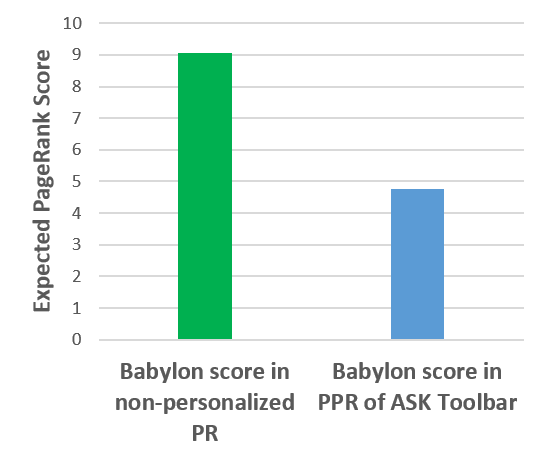
\includegraphics[scale=0.8]{figures/babylon_nosym_ask.png}
\caption{Babylon non-symbiotic relation with ASK Toolbar}
\label{fig:babylon_nosym_ask}
\end{subfigure}
\caption{Relationship between companies}
	\label{fig:symbiotic_pagerank}
\end{figure}

Personalized PageRank provides insights on a relation between Babylon and ASK (which are known rivals in the toolbar domain). In \autoref{fig:babylon_nosym_ask}, we see that Babylon's score decreases significantly in ASK's PPR, as compared to its score in non-personalized PageRank. Despite the fact that ASK and Babylon heavily co-occur in our dataset (see~\autoref{subsub:co_occurrence}), our result shows that there is no symbiotic relationship between the two companies. 

More symbiotic relations are shown in~\autoref{fig:symbiotic_2}. \autoref{fig:hotspot_sym_conduit} shows that HotSpot Shield is in symbiosis with Conduit, and this relationship can be verified in the Web\footnote{\url{https://www.pcrisk.com/removal-guides/7246-remove-hotspot-shield-toolbar}}. \autoref{fig:ask_sym_avira} shows a rather unusual partnership between an antivirus company Avira and the addon distributor ASK. When investigating relationships between antivirus companies and addons distributors, we see that addon distributor scores usually suffer in PPRs of antivirus companies, see \autoref{fig:ask_clash_trend}. A simple explanation is that some browser addons are considered malware and are removed by antivirus products. Nevertheless, in \autoref{fig:ask_sym_avira}, we observe that ASK toolbar's score increases in Avira's PPR. An explanation can be found on Avira's official web site, which states that ``Avira chose Ask.com to be our partner in bringing you the SearchFree Toolbar \dots''\footnote{\label{avira_ask}\url{https://www.avira.com/en/avira-searchfree-toolbar}}. 

\begin{figure}[!htbp]
\centering
\begin{subfigure}[b]{0.8\textwidth}
	\centering
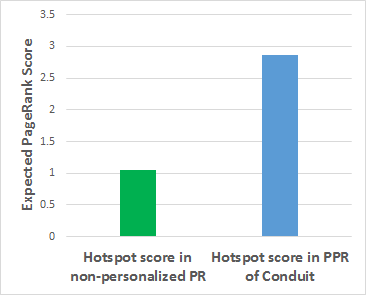
\includegraphics[scale=0.8]{figures/hotspot_sym_conduit.png}
\caption{Hotspot symbiotic relation with Conduit}
\label{fig:hotspot_sym_conduit}
\end{subfigure}
\begin{subfigure}[b]{0.8\textwidth}
	\centering
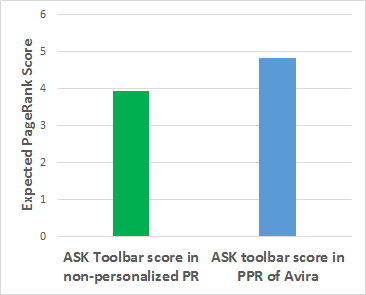
\includegraphics[scale=0.8]{figures/ask_sym_avira.png}
\caption{ASK Toolbar symbiotic relation with Avira}
\label{fig:ask_sym_avira}
\end{subfigure}
\caption{Symbiotic relations between companies}
	\label{fig:symbiotic_2}
\end{figure}

The most interesting symbiotic relationships are those that cannot be validated in the Web. For example, SearchToolbar appears symbiotic with a few companies, with the highest PPR to PR score ratios for Softonic and SweetIM. SearchToolbar is being manufactured by Zugo which is a small private company whose partnership agreements are not publicly disclosed. However, our results show that the existence of such agreements is quite apparent.

%\autoref{fig:incredi_sym_blekko} illustrates a symbiosis between Incredimail and Blekko. This discovery has an online reference\footnote{\url{http://www.im-infected.com/hijacker/blekko-search.html}}. As shown in \autoref{fig:blekko_sym_incredi}, this relationship is mutual: Blekko also benefits from this symbiosis, as well as Incredimail. 

%IncrediMail (Perion) and Conduit

%Avtiviruses bring other antiviruses down

%Zugo, SearchToolbar and SweetIM going together

%The same relationship is detected for Babylon and Conduit, see \autoref{fig:babylon_sym_conduit}, and again there is more than one online resource indicating the same. For example, Babylon addon named \emph{tbmyba.dll} is a Conduit Toolbar component\footnote{\url{http://www.file.net/process/tbmyba.dll.html}}. In fact, Conduit is known as a Toolbar manufacturer for other companies.


\subsection{Clash Relationships}
\label{sec:clash_relations}

In \autoref{sec:symb_relations}, we investigated symbiotic relationships between addon species, i.e. when one species benefit from another. In this section, we look for the opposite type of relationship: the \emph{clash}, which occurs when one species causes harm to another species. The idea behind detecting clash relations is very similar to the idea behind detecting simbiotic relations (as described in \autoref{sec:symb_relations}): we again aggregate addon PageRank scores into company scores --- both for non-personalized PagerRank and personalized PageRank with a query of all company's addons. In contrast to looking for companies whose scores increase, which we assume correspond to symbiotic relations, we now look for companies whose scores decrease substantially when another company is in the PPR query. 

As we can see in~\autoref{fig:RatioMatrix}, the company that experiences the most substantial plunge in the PPR to PR score ratios is the Norton Antivirus. Other antivirus companies such as AVG, Avira, and Kaspersky clash strongly with Norton. A fairly straightforward validation for these results comes from the fact that there is a known competition between antivirus companies: in most cases, two antivirus software products cannot coexist on the same computer, so when one product gets installed the other often gets uninstalled. Norton is known for being preinstalled on many computers, while cheaper antivirus software such as AVG replaces Norton at a later stage. This is precisely the phenomenon we observe in our results.

In the toolbar domain, it is remarkable to see that Google Toolbar appears clashing with all the other toolbars: smaller toolbar producers are likely to aim at uninstalling Google Toolbar as they consider Google their main competitor.

Let us show a few other examples. \autoref{fig:ask_clash_trend} shows that when an antivirus company TrendMicro is in the query, it causes ASK's scores to drop. Since antivirus companies sometimes treat toolbars as malware, this clash is not surprising. Another clash is shown in \autoref{fig:ask_clash_imesh}, between ASK and iMesh --- both companies operate in the toolbar space and are likely to compete with each other, however our result appears to be the only empirical proof for this competition.


\begin{figure}[!htbp]
\centering
\begin{subfigure}[b]{0.8\textwidth}
	\centering
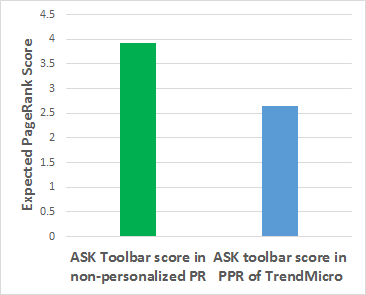
\includegraphics[scale=0.8]{figures/ask_clash_trend.png}
\caption{ASK Toolbar clash relation with TrendMicro}
\label{fig:ask_clash_trend}
\end{subfigure}
\begin{subfigure}[b]{0.8\textwidth}
	\centering
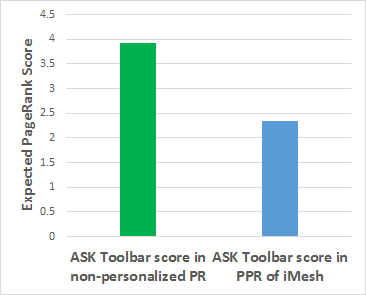
\includegraphics[scale=0.8]{figures/ask_clash_imesh.png}
\caption{ASK Toolbar clash relation with iMesh}
\label{fig:ask_clash_imesh}
\end{subfigure}
\caption{Clash relations between companies}
	\label{fig:clash_1}
\end{figure}

\iffalse
\begin{figure}[!htbp]
\centering
\begin{subfigure}[b]{0.8\textwidth}
	\centering
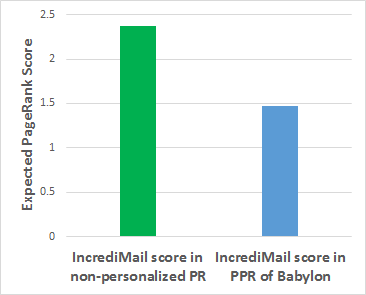
\includegraphics[scale=0.8]{figures/incredi_clash_babylon.png}
\caption{Incredimail clash relation with Babylon}
\label{fig:incredi_clash_babylon}
\end{subfigure}
\begin{subfigure}[b]{0.8\textwidth}
	\centering
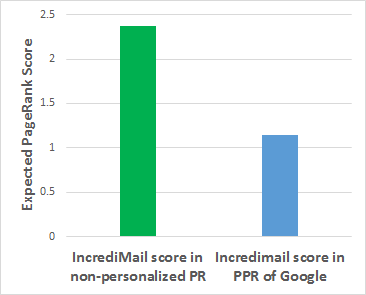
\includegraphics[scale=0.8]{figures/incredi_clash_google.png}
\caption{Incredimail clash relation with Google Toolbar}
\label{fig:incredi_clash_google}
\end{subfigure}
\caption{Clash relations between companies}
	\label{fig:clash_2}
\end{figure}
\fi

%A fairly straightforward validation for these results comes from the fact that there is a known competition between antivirus companies: in most cases, two antivirus software products can not coexist on the same computer, so when one product gets installed the other has to stop working and often gets uninstalled. Thus, using our terminology, antivirus companies stay in a clash relationship. And indeed, as shown in \autoref{fig:clash_av}, our algorithm detects antivirus companies clashing.

%Another clash relations is shown in \autoref{fig:clash_2}, we see that IncrediMail clashes with both Google Toolbars and Babylon. These three companies indeed competed (back in 2013) over toolbar installation on users machines. \autoref{fig:ask_clash_imesh} shows a clash between ASK toolbar and iMesh 

%[SELA: Added clash between ASK toolbar and iMesh \autoref{fig:ask_clash_imesh}]
\iffalse
\begin{figure}[!htbp]
\centering
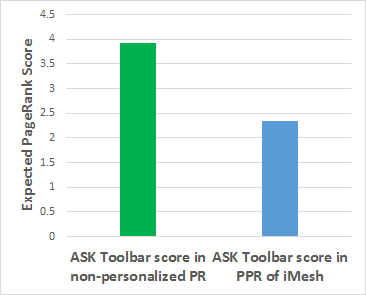
\includegraphics[scale=0.8]{figures/ask_clash_imesh.png}
\caption{ASK Toolbar relationship with iMesh}
\label{fig:ask_clash_imesh}
\end{figure}

\begin{sidewaysfigure}[!ht]
    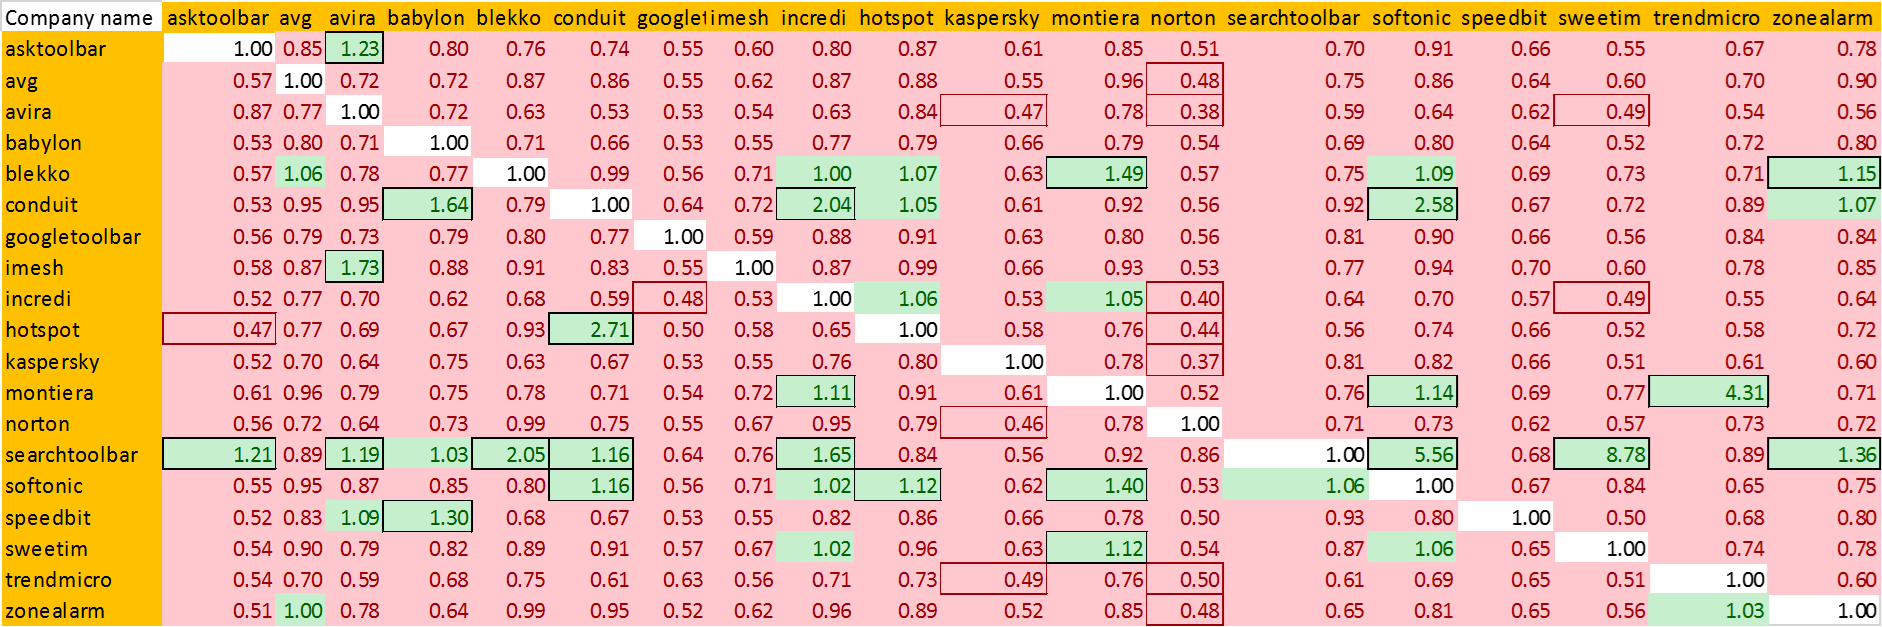
\includegraphics[scale=0.8]{figures/RatioMatrix.png}
    \caption{Expected PPR and PR ratio between the companies}
    \label{fig:RatioMatrix}
\end{sidewaysfigure}

\begin{figure}[!htbp]
\centering
\begin{subfigure}[b]{0.49\textwidth}
	\centering
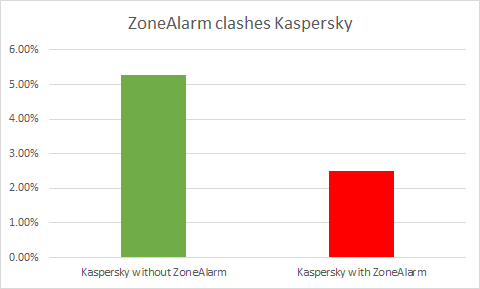
\includegraphics[scale=0.49]{figures/zone_clash_kaspersky.png}
\caption{ZoneAlarm clash relationship with Kaspersky}
\label{fig:zone_clash_kaspersky}
\end{subfigure}
\begin{subfigure}[b]{0.49\textwidth}
	\centering
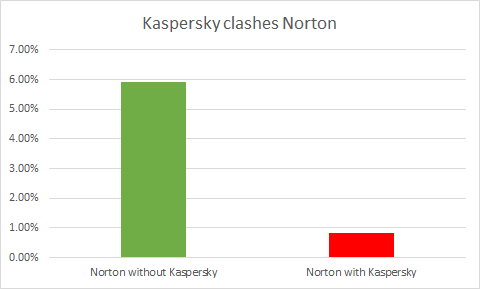
\includegraphics[scale=0.49]{figures/kaspersky_clash_norton.png}
\caption{Kaspersky clash relationship with Norton}
\label{fig:kaspersky_clash_norton}
\end{subfigure}
\caption{Clash relationship between AntiVirus companies}
	\label{fig:clash_av}
\end{figure}

\begin{figure}[!htbp]
\centering
\begin{subfigure}[b]{0.8\textwidth}
	\centering
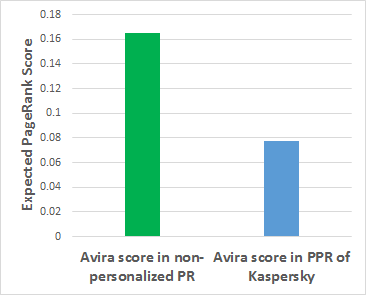
\includegraphics[scale=0.8]{figures/avira_clash_kaspersky.png}
\caption{Avira clash relationship with Kaspersky}
\label{fig:avira_clash_kaspersky}
\end{subfigure}
\begin{subfigure}[b]{0.8\textwidth}
	\centering
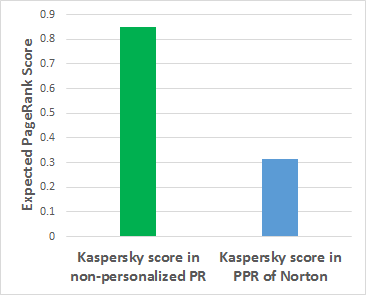
\includegraphics[scale=0.8]{figures/kaspersky_clash_norton_2.png}
\caption{Kaspersky clash relationship with Norton}
\label{fig:kaspersky_clash_norton}
\end{subfigure}
\caption{Clash relationship between AntiVirus companies}
	\label{fig:clash_av}
\end{figure}
\fi

\iffalse
After aggregating all add-ons for each for every company we have looked for what have happened to other company add-ons when PPR origin is a specific company.
For example, we have looked at HotSpot company and the impact it has on other companies.\\
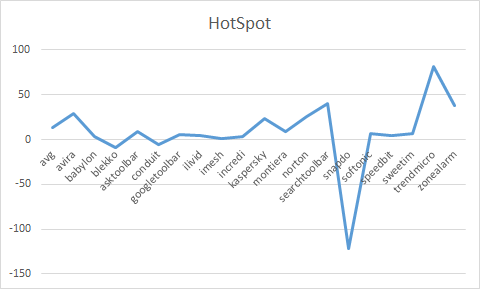
\includegraphics[scale=1.0]{hotspot.png}\\
As we can see from the chart some companies like trendmicro has a symbiosis with hotspot add-ons. While other companies, like SnapDo, are clashing with HotSpot add-ons.
This analysis, is even more interesting in light of recent security breach with Superfish and Komodia. After this security breach was identified, security researches where looking for more companies that have cooperated with Komodia. We believe that given that data, our algorithm would identify these companies as having a symbiosis with Komodia.
\fi

\iffalse
First, we needed some basic ranking of all add-ons from all companies, we believe that regular PageRank scores on this graph provide a good base line to all add-ons metrics. [Why do we need basic rankings? - RON][SELA] Basic ranking it is actually a baseline ranks, we were running a regular pagerank for this. It was used as a baseline, afterwards, for comparing how the rank of company addons has increased/decreased. BTW, this text is not in the thesis...
Then, we identified add-ons belonging to a company by looking for the company's name in addon descriptions. But what if the addon does not contain the company's name, can we still identify it as related to the company? To solve this problem, we applied an approach similar to the one we used to identify a "missing" addon. We ran PPR from all known add-ons of a specific company (for example, Babylon), and looked at all add-ons that drastically improved its rank compared to its previous rank given by PageRank.
By searching the addon names in the Web, many of them were found to be related to the company that originated the PPR (whose add-ons composed the PPR vector). For example,an  addon named tbmyba.dll, jumped from the 1200 rank position to the 15 rank position when running PPR from Babylon, and indeed we found that this addon is related to Babylon. 
After identifying all company add-ons, we decided to remove add-ons that are installed at fewer than 100 users' machines: these add-ons seemed to have almost no impact on the results but have made more difficult to look for tendencies between firms. [Why is that? - RON] [SELA] There were many addons that was installed only on few machines, we wanted to try to look at the addons "manually" and understand what is going on. Since the addons on small amount of machines did not have any impact, we could just remove them.\\
\fi


\section{Conclusion}
\label{sec:clash_conclusion}
In this chapter, we had an ambitious goal to analyze the global ecosystem of Web browser addons over a large sample of almost a million personal computers. After developing the analytics toolkit in \autoref{chap:user_ecosystem} and empirically proving the correctness of developed algorithms at the individual level, in this chapter we took the developed methodology to the macro-level.
We were looking for a way to discover mostly hidden relationships between the addons manufacturing companies, and were pleased to discover that the tools from \autoref{chap:user_ecosystem} can come handy here as well.

First, we developed a method for mapping addons to their manufacturers that went beyond a straightforward search for a company name in the addon attributes. The problem of mapping addons to their manufacturers is important in security applications. Using personalized PageRank centered around known addons of a company, we discovered that most addons of the same manufacturer form a kind of community: once some addons of the same manufacture are climbing up in the PR scores - all addons of that manufacture will climb up, the discussion of this behavior is in \autoref{sec:experiment_des}.
After we chose 19 known addons manufactures and their related addons, we looked for the relations betweem them.
After careful consideration, we decided that weighted aggregation of each company addons scores is the correct way to represent the companies in future analysis.
We looked at all companies through the lens of every standalone company - checking companies scores changes given the presence of some individual company.
In \autoref{sec:symb_relations}, we discovered a symbiotic relations between some of the given company. We were amazed to see that every relation we discovered is grounded in reality. Some of the symbiotic relations were so surprising, like a symbiotic relation between antivirus company and addon developer (a natural rivals), that we double checked the results and were proven correct. Interestingly, the justifications for our results we found in the web, using Google's search engine - based on PageRank.

In \autoref{sec:clash_relations}, we looked at the opposite of symbiotic relations -  a clash relations. For this kind of relations, we found an additional way to validate our measurements - it is a well known fact the antivirus companies clash (two antivirus products cannot be installed on the same machine). This relations between the antivirus companies were discovered by our technique in addition to other companies relations as well.

In this chapter, we found and proved a methodology to find typically hidden relations between companies as well as related unknown addons to its manufactures.

%We are comparing for each company its total weighted rank in PageRank with its total weighted rank in Personalized PageRank when another company is the PPR vector.
%We have found that there are companies that co-exist well with other companies, there are even companies that improve greatly other companies add-ons rank.
%We have also observed companies that cause other companies add-ons decline.

\chapter{Summary of contributions}
\label{chap:summary}
Web Browser addons is an unresearched domain. In this work we aimed at developing tools and methodology for addons behavioral analysis.
Given an unique dataset of addons, we practiced different types of data layering and collection, and different types of machine learning algorithms until we came up with the final decision about how to organize the data for a future analysis, this process is described in \autoref{sec:datasets}.
After organizing the data in a graph of users and addons, knowing that Personalized PageRank is well-suited for capturing relationships between vertices in a graph, we proposed the PPR as the basis for analysing the addons behaviour.
Believing that user addons for some kind of an ecosystem with its own rules, we believed that since such rules exist we can conjectured that we can predict the addons behaviour.
At first, we have looked for a way to predict which addons is missing at user addons ecosystem, given all other user addons.
Our algorithm would output a ranked list of addons it finds the most appropriate to appear at the given user, already in the first experiment we had an impressive results - the predicted addon, with high probability, was found in top 10 in the ranked list. In \autoref{chap:user_ecosystem}, we describe the many experiments we conducted while searching for optimized setup. Given the "Big Data" size of the graph, we had to overcome the technical difficulty in order to run many thousands of experiments in suitable amount of time.
As the results show in \autoref{chap:user_ecosystem}, our approach significantly outperforms all the baselines.
While an extensive work with addons in \autoref{chap:user_ecosystem}, some interesting phenomena poped-up, we saw that not only addons have a relations via user but also addons have a relations between them based on their company manufacture. We saw that some addons appear more with some addons and seems to not appear at all with some other addons.
Armed with this observation and with the methodology from \autoref{chap:user_ecosystem}, we decided to explore this phenomena more deeply, and maybe shed light on the relations between addons manufactures.
In \autoref{chap:Symbiosis}, we explore these relations between the addon companies.
We discovered that some companies are having a symbiotic relations - when one company addon are installed there is a good chance that the other company addons will be there too. Moreover, we discovered that simple co-occurrence measure is not good enough to indicate a symbiotic relations - while our methodology is very precise when discovering symbiosis between companies. Given the symbiotic relations, as one would have guessed, we also discovered the opposite relations between companies - we coined it as a clash relations.
In the clash relations, addons of one company do not tend to appear with addons of another company. Our discoveries about the companies were justified by looking at press releases and by learning to understand the way specific companies are operating.
While working on \autoref{chap:Symbiosis}, we have also discovered a way relate an addon to a company even when its attributes have no clue that this addon may be related to a specific company, the algorithm described in \autoref{chap:Symbiosis}.

To conclude, working with a unique domain with no prior research on Browser addons conducted, we have successfully build a toolset and methodology to deal with this domain.
We have developed an algorithm that predicts a missing user addon and significantly outperforms the baseline algorithms.
We have discovered and correctly predicted a relationships between addons manufacture companies.



%\bibliographystyle{alpha}
\iffalse
\newpage
\appendix
\chapter{} 
\renewcommand{\figurename}{Appendix}

\begin{figure}[!htbp]
\centering
\begin{subfigure}[b]{0.49\textwidth}
	\centering
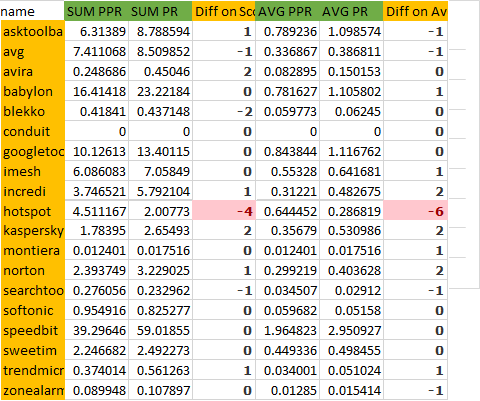
\includegraphics[scale=0.49]{figures/conduit_pr_scores.png}
\end{subfigure}
\begin{subfigure}[b]{0.49\textwidth}
	\centering
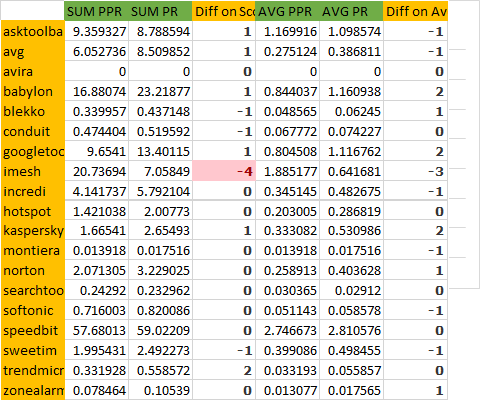
\includegraphics[scale=0.49]{figures/avira_pr_scores.png}
\end{subfigure}
\caption{PR scores}
	\label{fig:appendix_pr}
\end{figure}

\begin{figure}[!htbp]
\centering
\begin{subfigure}[b]{0.49\textwidth}
	\centering
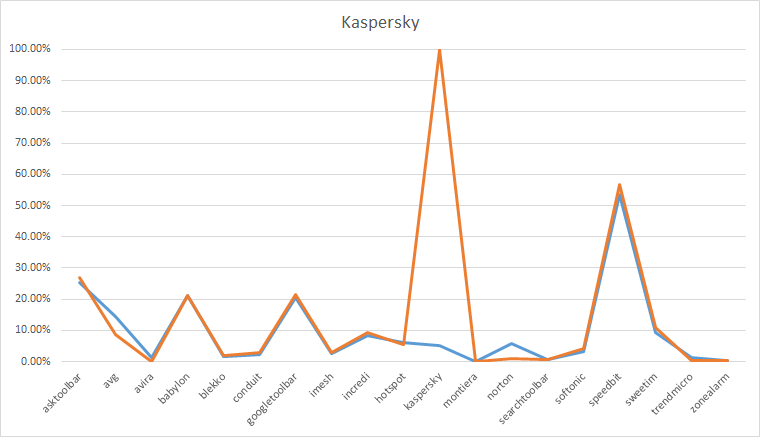
\includegraphics[scale=0.49]{figures/kaspersky_graph.png}
\end{subfigure}
\begin{subfigure}[b]{0.49\textwidth}
	\centering
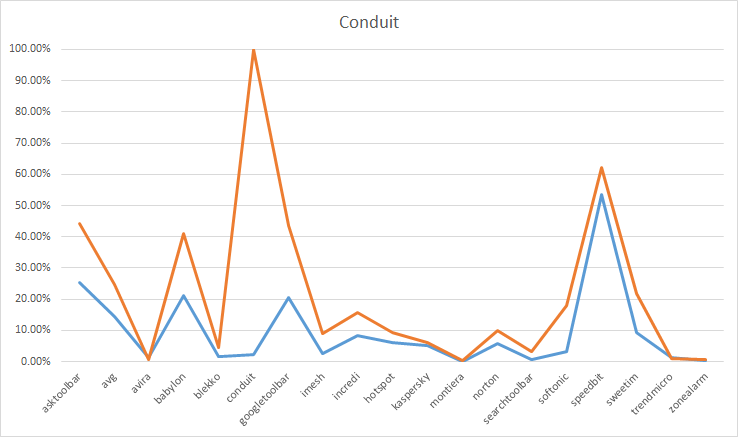
\includegraphics[scale=0.49]{figures/conduit_graph.png}
\end{subfigure}
\caption{Graph scores}
	\label{fig:appendix_pr2}
\end{figure}

\begin{figure}[!htbp]
\centering
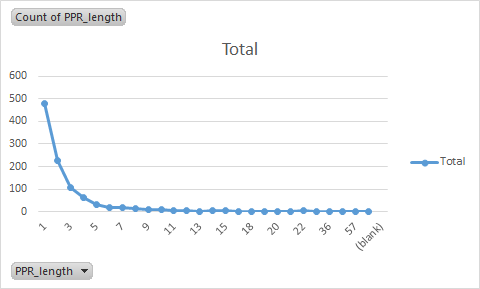
\includegraphics[scale=0.8]{figures/PPR_length_dist.png}
\caption{Personaliztion vector length}
\end{figure}
\fi


\bibliographystyle{apalike}
\bibliography{thesisdraft}
\addcontentsline{toc}{chapter}{Bibliography}

\end{document}

